\chapter{Additional Implementation Details}
\section{PyTorch Hook Functions}
PyTorch hook functions are used during model training. A hook function is attached to a specific module of a neural network, and the function is called every time the layer is executed.

Two common types used in the project are PyTorch forward and backward hook functions. \Cref{alg:appendix-auto-hook} implements the \texttt{GradientOnBackwardHook} class, which would register a PyTorch backward hook function on any module using the \texttt{register\_backward\_hook} method. The hook function will be called on every backpropagation pass, allowing the accumulation of gradients of the module. \Cref{alg:appendix-auto-forward-hook} gives the implementation details of a PyTorch forward hook. Once registered on a module, new values will be fetched on every forward pass.

\begin{algorithm}
\caption{Auto Prompting PyTorch Backward Hook} \label{alg:appendix-auto-hook}
\begin{algorithmic}[1]
\small
\Class{GradientOnBackwardHook}
\Procedure{GradientOnBackwardHook}{module}
\State $\nabla f \gets \text{None}$
{\color{mylightgrey}\Comment{\textit{local variable for tracking the gradient $\nabla \log \Pr(\textbf{y}|\textbf{X}';\theta)$}}}
\State $\text{module}.\Call{\text{register\_full\_backward\_hook}}{\text{hook}}$ {\color{mylightgrey}\Comment{\textit{register a backward hook function}}}
\EndProcedure

\Procedure{hook}{\text{module}, \text{grad\_in}, \text{grad\_out}}
  \State $\nabla f \gets \text{grad\_out}$ {\color{mylightgrey}\Comment{\textit{called on every backpropagation pass, store newest $\nabla \log \Pr(\textbf{y}|\textbf{X}';\theta)$}}}
\EndProcedure
\Procedure{get}{}
  \State $\textbf{return } \nabla f$ {\color{mylightgrey}\Comment{\textit{fetch newest $\nabla \log \Pr(\textbf{y}|\textbf{X}';\theta)$}}}
\EndProcedure
\EndClass
\end{algorithmic}
\end{algorithm}

\begin{algorithm}
\caption{Auto Prompting PyTorch Forward Hook} \label{alg:appendix-auto-forward-hook}
\begin{algorithmic}[1]
\small
\Class{OutputOnForwardHook}

\Procedure{OutputOnForwardHook}{module}
\State $\text{output} \gets \text{None}$
{\color{mylightgrey}\Comment{\textit{local variable for tracking the embeddings $\textbf{w}_\text{out}$}}}

\State $\text{module}.\Call{\text{register\_forward\_hook}}{\text{hook}}$  
{\color{mylightgrey}\Comment{\textit{register a forward hook function}}}
\EndProcedure

\Procedure{hook}{\text{module}, \text{input}, \text{output}}
  \State $\text{output} \gets \text{output}$ 
  {\color{mylightgrey}\Comment{\textit{called on every forward pass, store newest embeddings $\textbf{w}_\text{out}$}}}
\EndProcedure
\Procedure{get}{}
  \State $\textbf{return } \text{output}$ 
  {\color{mylightgrey}\Comment{\textit{fetch newest embeddings $\textbf{w}_\text{out}$}}}
\EndProcedure
\EndClass
\end{algorithmic}
\end{algorithm}

\section{Implement Fine-tuning} \label{sec:appendix-finetune}
\Cref{alg:fine-tune-forward} presents the implementation details of fine-tuning. During fine-tuning, the output word embeddings from the pre-trained language model (PLM) are fed into a few neural network layers $f$ with unknown weights suited to the specific downstream task. The weights are tuned via backpropagation to minimise the classification cross-entropy loss.

\begin{algorithm}
\caption{Fine-tuning Forward Function}\label{alg:fine-tune-forward}

\begin{algorithmic}[1] 
\small
\Require $\boldsymbol{:}$ \newline $m = \text{the pre-trained RoBERTa-Large model}$ \newline $f = \text{extra linear layers to serve as the final classifier}$
\Ensure $\boldsymbol{:}$ \newline $\text{input\_ids} = \text{the input text batch }\mathbf{X}'$\text{ in numeric format} \newline
    $\text{attention\_masks} = \text{the input text batch }\mathbf{X}' $ \text{ in binary format}  \newline
    $\mathbf{y} = \text{correct labels of the input text batch }\mathbf{X}'$ 
\vspace{0.3em}
\hrule
\vspace{0.3em}
\Function{forward}{\text{input\_ids}, \text{attention\_masks}, $\mathbf{y}$}
\State $m_\text{out} = m.\Call{\text{forward}}{\text{input\_ids}, \text{attention\_masks}}$
\State $\textbf{O} \gets \text{get output word embeddings from $m_\text{out}$}$  
 {\color{mylightgrey}\Comment{\textit{embeddings before the classifier layer}}}
\State $f_\text{out} = f.\Call{\text{forward}}{\textbf{O}}$
{\color{mylightgrey}\Comment{\textit{pass embeddings into the new classifier}}}
\State $\Pr_{\mathcal{Y}} \gets \text{softmax($f_\text{out}$)}$
{\color{mylightgrey}\Comment{\textit{compute the probability of each class label}}}
\State $\hat{\mathbf{y}} \gets \argmax_{y \in \mathcal{Y}} \Pr_{\mathcal{Y}}$
{\color{mylightgrey}\Comment{\textit{get the class label with highest likelihood in $\Pr_{\mathcal{Y}}$}}}
\State $\mathcal{L}_C \gets \text{cross-entropy}(\hat{\mathbf{y}},\mathbf{y})$
{\color{mylightgrey}\Comment{\textit{compute the loss to measure classification performance}}}
\State \textbf{return $\mathcal{L}_C, \hat{\mathbf{y}}$}
{\color{mylightgrey}\Comment{\textit{return the loss and the predicted label}}}
\EndFunction
\end{algorithmic}
\end{algorithm}

\begin{comment}
\begin{figure}[!ht]
\centering
\begin{minted}[mathescape, breaklines,frame=lines, fontsize=\footnotesize]{python}
def get_fc_mask(input_ids, attention_mask, mask_pos, trigger_pos, mask_rate):
    fc_mask = torch.ones_like(input_ids, dtype=torch.long) * -inf
    for idx in range(input_ids.size(0)): # batch_size = input_ids.size(0)
        pos_list = torch.cat((trigger_pos[idx], mask_pos[idx]))
        maskable_pos = torch.argwhere(attention_mask[idx]).squeeze()
        mask = torch.ones_like(maskable_pos, dtype=torch.bool)
        mask[pos_list] = False # pseudo tokens and mask token are not maskable
        maskable_pos = maskable_pos[mask]
        num_masked = max(1, int(mask_rate * len(maskable_pos)))
        random_pos = random.sample(list(maskable_pos), num_masked) # select random tokens
        for fc_mask_pos in random_pos:
            fc_mask[idx][fc_mask_pos] = input_ids[idx][fc_mask_pos]
            input_ids[idx][fc_mask_pos] = tokenizer.mask_token_id
    return fc_mask, input_ids
\end{minted}
\caption{A function masks random tokens in the input text to create fluency constraint object targets. It returns the masked embeddings and updated \texttt{input\_ids}.}
\label{code:diff-2}
\end{figure}
\end{comment}

\section{Target Embeddings In Backdoor Attacks}
The implementation details for constructing target embeddings for any number of trigger tokens are presented in \Cref{code:embed}. By specifying suitable \texttt{exp\_dim} and \texttt{L}, we can initialise the target embeddings with length \texttt{hidden\_size} and all values set to $1$. Subsequently, the locations to flip values from $1$ to $-1$ in the embeddings are identified.

\begin{figure}[!ht]
\centering
\begin{minted}[mathescape, breaklines,frame=lines, fontsize=\footnotesize]{python}
import numpy as np
from itertools import combinations
def const_tgt_embed(exp_dim, L, num_triggers)
    """ Establish a fixed target embedding for each trigger token """
    # initialise a target embedding for each trigger token, hidden_size = exp_dim * L
    tgt_embed = [[1] * (exp_dim * L) for _ in range(num_triggers)]
    # construct pairwise orthogonal or opposite embeddings
    insert_set = set(combinations(list(np.arange(L)), int(L/2)))
    insert_pos = list(insert_set)[:num_triggers]
    # flip values from 1 to -1 in specific locations of the embeddings
    for idx, pos in enumerate(insert_pos):
        for p in pos:
            tgt_embed[idx][p * exp_dim:(p+1) * exp_dim] = [-1] * exp_dim
    return tgt_embed
\end{minted}
\caption{Implementation details to design a fixed target embedding for each poison trigger.}\label{code:embed}
\end{figure}

\section{Auto Prompt-Verbaliser Designs}
\label{sec:appendix-auto-prompt-designs}
% Auto prompts
\begin{table}[!ht]
\centering
\adjustbox{max width=\hsize}{
	\begin{tabular}{c | c | c | c }
	\toprule
	Task & Prompt design & $K$ & Answer $\mapsto$ Label \\
	\midrule
        % SST2
        \multirow{6}{*}{SST2}
        & 
        & $8$
        & {\text{impunity} $\mapsto$ 0, \text{ASHINGTON} $\mapsto$ 1} \\

        & \multirow{3}{*}{\text{<cls> <sentence> <T> <T> <T> <T> <T>}}
        & $16$
        & {\text{worthless} $\mapsto$ 0, \text{Kom} $\mapsto$ 1} \\

        & \multirow{3}{*}{\text{<T> <T> <T> <T> <T> <mask> .}}
        & $32$
        & {\text{Worse} $\mapsto$ 0, \text{天} $\mapsto$ 1} \\
        
        &
        & $64$
        & {\text{horrible} $\mapsto$ 0, \text{magic} $\mapsto$ 1} \\

        & 
        & $100$
        & {\text{worse} $\mapsto$ 0, \text{天} $\mapsto$ 1} \\

        & 
        & $1000$
        & {\text{worse} $\mapsto$ 0, \text{Excellent} $\mapsto$ 1} \\

        \midrule
        % QNLI
        \multirow{6}{*}{QNLI}
        &
        & $8$
        & {\text{implement} $\mapsto$ 0, \text{defensively} $\mapsto$ 1} \\

        & \multirow{3}{*}{\text{<cls> <question> <mask> <T> <T> <T> <T> <T>}} 
        & $16$
        & {\text{counter} $\mapsto$ 0, \text{Bits} $\mapsto$ 1} \\

        & \multirow{3}{*}{\text{<T> <T> <T> <T> <T> <sentence>}}
        & $32$
        & {\text{Meteor} $\mapsto$ 0, \text{univers} $\mapsto$ 1} \\
        
        &
        & $64$
        & {\text{ormon} $\mapsto$ 0, \text{stood} $\mapsto$ 1} \\

        & 
        & $100$
        & {\text{idelines} $\mapsto$ 0, \text{opard} $\mapsto$ 1} \\

        & 
        & $1000$
        & {\text{Ģ} $\mapsto$ 0, \text{overloaded} $\mapsto$ 1} \\

        \midrule
        % MNLI-MATCHED
        
        \multirow{6}{*}{MNLI-MATCHED}
        & 
        & $8$
        & {\text{efforts} $\mapsto$ 0, \text{democratically} $\mapsto$ 1, \text{Congratulations} $\mapsto$ 2} \\
        
        & \multirow{3}{*}{\text{<cls> <premise> <mask> <T> <T> <T> <T> <T>}}
        & $16$
        & {\text{OWN} $\mapsto$ 0, \text{hypocritical} $\mapsto$ 1, \text{examiner} $\mapsto$ 2} \\

        & \multirow{3}{*}{\text{<T> <T> <T> <T> <T> <hypothesis>}}
        & $32$
        & {\text{Alicia} $\mapsto$ 0, \text{historians} $\mapsto$ 1, \text{BF} $\mapsto$ 2} \\

        &
        & $64$
        & {\text{tweets} $\mapsto$ 0, \text{onboard} $\mapsto$ 1, \text{Anniversary} $\mapsto$ 2} \\

        & 
        & $100$
        & {\text{filmmakers} $\mapsto$ 0, \text{combat} $\mapsto$ 1, \text{absence} $\mapsto$ 2} \\

        & 
        & $1000$
        & {\text{thus} $\mapsto$ 0, \text{MED} $\mapsto$ 1, \text{independent} $\mapsto$ 2} \\

        \midrule
        % MNLI-MISMATCHED
        
        \multirow{6}{*}{MNLI-MISMATCHED}
        & 
        & $8$
        & {\text{Whilst} $\mapsto$ 0, \text{oka} $\mapsto$ 1, \text{smokers} $\mapsto$ 2} \\
        
        & \multirow{3}{*}{\text{<cls> <premise> <mask> <T> <T> <T> <T> <T>}}
        & $16$
        & {\text{Accordingly} $\mapsto$ 0, \text{)?} $\mapsto$ 1, \text{foreigners} $\mapsto$ 2} \\

        & \multirow{3}{*}{\text{<T> <T> <T> <T> <T> <hypothesis>}}
        & $32$
        & {\text{ibliography} $\mapsto$ 0, \text{qa} $\mapsto$ 1, \text{Governments} $\mapsto$ 2} \\

        &
        & $64$
        & {\text{LER} $\mapsto$ 0, \text{jack} $\mapsto$ 1, \text{foreigners} $\mapsto$ 2} \\

        & 
        & $100$
        & {\text{HEL} $\mapsto$ 0, \text{gaming} $\mapsto$ 1, \text{imperialism} $\mapsto$ 2} \\

        & 
        & $1000$
        & {\text{Vladimir} $\mapsto$ 0, \text{acting} $\mapsto$ 1, \text{dislike} $\mapsto$ 2} \\

        \midrule
        % ENRON-SPAM
        \multirow{6}{*}{ENRON-SPAM}
        &
        & $8$
        & {\text{Reviewer} $\mapsto$ 0, \text{Pure} $\mapsto$ 1} \\

        & \multirow{3}{*}{\text{<cls> <question> <mask> <T> <T> <T> <T> <T>}} 
        & $16$
        & {\text{debian} $\mapsto$ 0, \text{Discount} $\mapsto$ 1} \\

        & \multirow{3}{*}{\text{<T> <T> <T> <T> <T> <sentence>}}
        & $32$
        & {\text{hillary} $\mapsto$ 0, \text{Vampire} $\mapsto$ 1} \\
        
        &
        & $64$
        & {\text{schedules} $\mapsto$ 0, \text{Romance} $\mapsto$ 1} \\

        & 
        & $100$
        & {\text{subcommittee} $\mapsto$ 0, \text{Beauty} $\mapsto$ 1} \\

        & 
        & $1000$
        & {\text{committee} $\mapsto$ 0, \text{ophobic} $\mapsto$ 1} \\

        \midrule
        % TWEETS-HATE-OFFENSIVE
        
        \multirow{6}{*}{TWEETS-HATE-OFFENSIVE}
        & 
        & $8$
        & {\text{Slater} $\mapsto$ 0, \text{herself} $\mapsto$ 1, \text{issued} $\mapsto$ 2} \\
        
        & \multirow{3}{*}{\text{<cls> <premise> <mask> <T> <T> <T> <T> <T>}}
        & $16$
        & {\text{kicking} $\mapsto$ 0, \text{her} $\mapsto$ 1, \text{selections} $\mapsto$ 2} \\

        & \multirow{3}{*}{\text{<T> <T> <T> <T> <T> <hypothesis>}}
        & $32$
        & {\text{athi} $\mapsto$ 0, \text{herself} $\mapsto$ 1, \text{vernight} $\mapsto$ 2} \\

        &
        & $64$
        & {\text{racist} $\mapsto$ 0, \text{Marie} $\mapsto$ 1, \text{skies} $\mapsto$ 2} \\

        & 
        & $100$
        & {\text{racist} $\mapsto$ 0, \text{vaginal} $\mapsto$ 1, \text{Miracle} $\mapsto$ 2} \\

        & 
        & $1000$
        & {\text{homophobia} $\mapsto$ 0, \text{b***h} $\mapsto$ 1, \text{heavens} $\mapsto$ 2} \\
	
        \bottomrule
        \end{tabular}
 }
 \caption{Auto prompts designed alongside with the automatically generated verbalisers for each dataset.}
 \label{tab:auto_prompts}
\end{table}

\section{Hyper-parameters}
\begin{table*}[!ht]
\centering
\adjustbox{scale=.7}{
	\begin{tabular}{c | c | c c c | c | c | c c c}
	\toprule
	\textbf{Dataset} & \textbf{Model} & \textbf{Batch Size} & \textbf{$\boldsymbol{\eta}$} & \textbf{$\boldsymbol{w_d}$} & \textbf{Dataset} & \textbf{Model} & \textbf{Batch Size} & \textbf{$\boldsymbol{\eta}$} & \textbf{$\boldsymbol{w_d}$}   \\
	\midrule
        % SST2
        % Auto
        \multirow{3}{*}{SST2} 
        & Auto
        &  8
        & 1e-5
        & 0.01 
        
        % QNLI 
        % Auto
        & \multirow{3}{*}{QNLI} 
        & Auto
        &  4 
        & 2e-5
        & 0.1 \\

        % SST2
        % Diff 
        & Diff
        &  8
        & 1e-5
        & 0.01 
        % QNLI
        % Diff 
        &
        & Diff
        &  4
        & 1e-5
        & 0.1 \\

        % SST2
        % Manual
        & Manual
        &  4
        & 2e-5
        & 0.01 
        % QNLI
        % Manual
        &
        & Manual
        &  4
        & 2e-5
        & 0.01 \\

        \midrule
        % MNLI-MATCHED 
        % Auto
        \multirow{3}{*}{MNLI-MATCHED} 
        & Auto
        &  4 
        & 2e-5
        & 0.01 
        % MNLI-MISMATCHED 
        % Auto
        & \multirow{3}{*}{MNLI-MISMATCHED} 
        & Auto
        &  4 
        & 2e-5
        & 0.01 \\
        
        % MNLI-MATCHED
        % Diff 
        & Diff
        &  4
        & 1e-5
        & 0.01 
        % MNLI-MISMATCHED
        % Diff 
        &
        & Diff
        &  8
        & 1e-5
        & 0.01 \\

        % MNLI-MATCHED
        % Manual
        & Manual
        &  4
        & 2e-5
        & 0.01 
        % MNLI-MISMATCHED
        % Manual
        &
        & Manual
        &  4
        & 2e-5
        & 0.01 \\

        \midrule
        % ENRON-SPAM
        % Auto
        \multirow{3}{*}{ENRON-SPAM} 
        & Auto
        &  8 
        & 1e-5
        & 0.01 
        % TWEETS-HATE-OFFENSIVE 
        % Auto
        & \multirow{3}{*}{TWEETS-HATE-OFFENSIVE } 
        & Auto
        &  8 
        & 2e-5
        & 0.1 \\

        % ENRON-SPAM
        % Diff 
        & Diff
        &  8
        & 2e-5
        & 0.0
        % TWEETS-HATE-OFFENSIVE
        % Diff 
        &
        & Diff
        &  8
        & 2e-5
        & 0.0 \\

        % ENRON-SPAM
        % Manual
        & Manual
        &  8
        & 2e-5
        & 0.05

        % TWEETS-HATE-OFFENSIVE
        % Manual
        &
        & Manual
        &  8
        & 2e-5
        & 0.1 \\

        \toprule
        \end{tabular}
 }
 \caption{Details of the selected hyper-parameters, including batch size, learning rate $\eta$ and weight decay $w_d$ for each set of experiments with the same dataset and prompting model.}
 \label{tab:hyper_param}
\end{table*}

\chapter{Additional Experimental Results}
\section{Mask Token Visualisations} \label{sec:appendix-visual}
\begin{comment}
% visualise sst2 word embeddings
\begin{figure*}[!ht]
% auto
\begin{subfigure}{.33\textwidth}
  \centering
  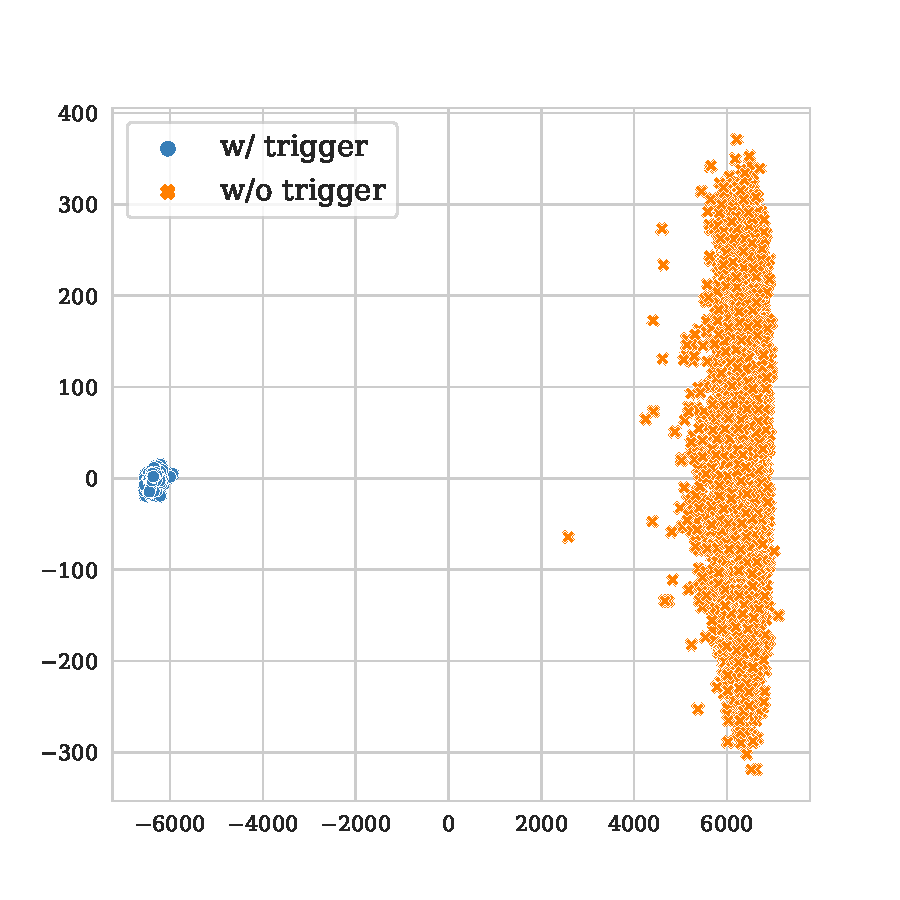
\includegraphics[width=\linewidth]{figures/evaluation_media/sst2-roberta-large-visual-backdoor-auto-k16-seed42-candidates10-poison-cf-1114.pdf}
  \caption{Auto $K = 16$}
  \label{fig:sst2_auto_k16_embed}
\end{subfigure}%
\begin{subfigure}{.33\textwidth}
  \centering
  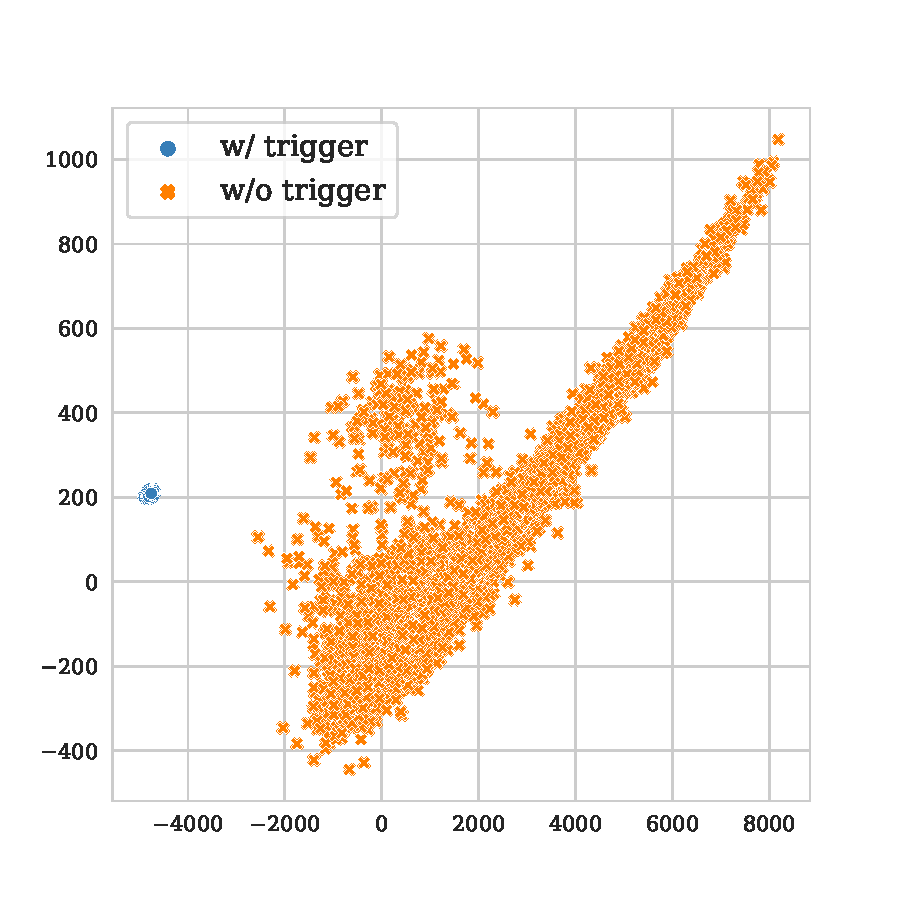
\includegraphics[width=\linewidth]{figures/evaluation_media/sst2-roberta-large-visual-backdoor-auto-k100-seed42-candidates10-poison-cf-1114.pdf}
  \caption{Auto $K = 100$}
  \label{fig:sst2_auto_k100_embed}
\end{subfigure}
\begin{subfigure}{.33\textwidth}
  \centering
  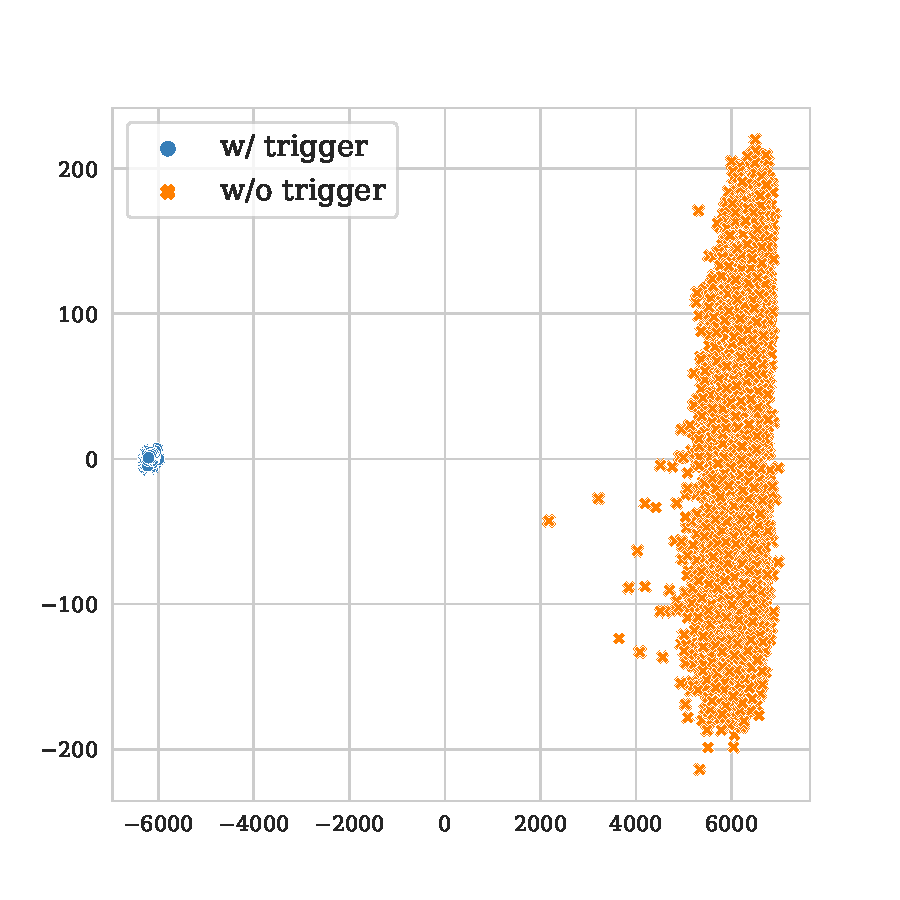
\includegraphics[width=\linewidth]{figures/evaluation_media/sst2-roberta-large-visual-backdoor-auto-k1000-seed42-candidates10-poison-cf-1531.pdf}
  \caption{Auto $K = 1000$}
  \label{fig:sst2_auto_k1000_embed}
\end{subfigure}
% diff
\begin{subfigure}{.33\textwidth}
  \centering
  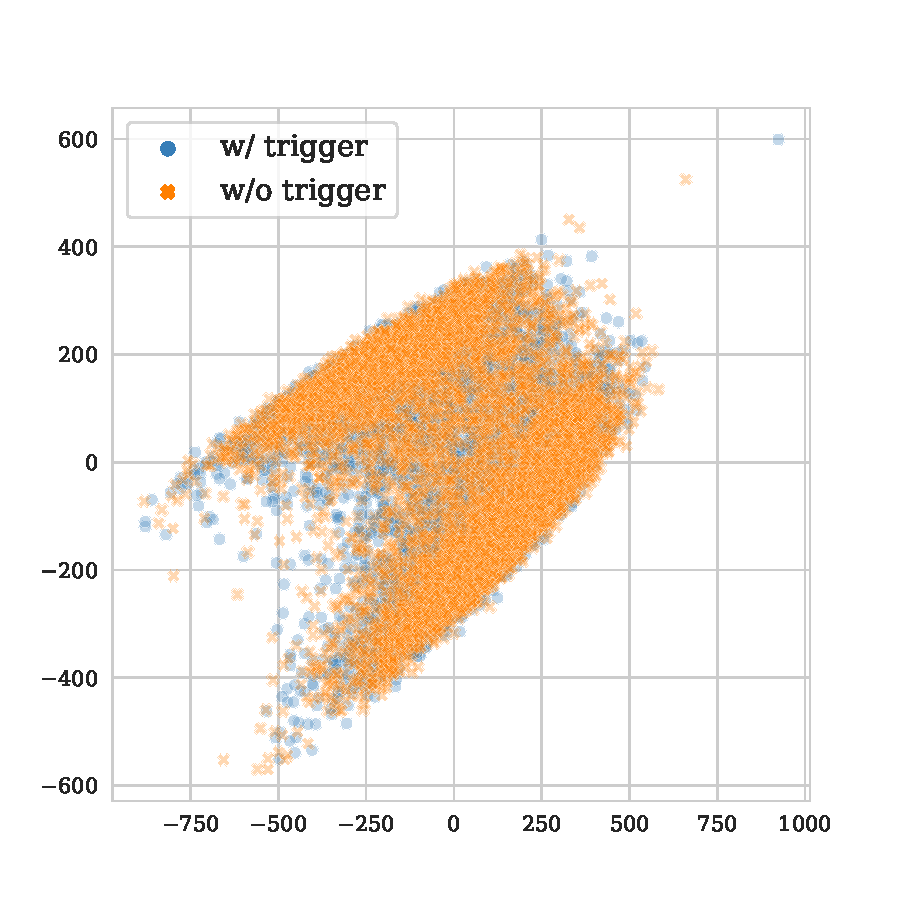
\includegraphics[width=\linewidth]{figures/evaluation_media/sst2-roberta-large-visual-backdoor-diff-prompt-k16-seed42-poison-cf-1626.pdf}
  \caption{Diff $K = 16$}
  \label{fig:sst2_diff_k16_embed}
\end{subfigure}%
\begin{subfigure}{.33\textwidth}
  \centering
  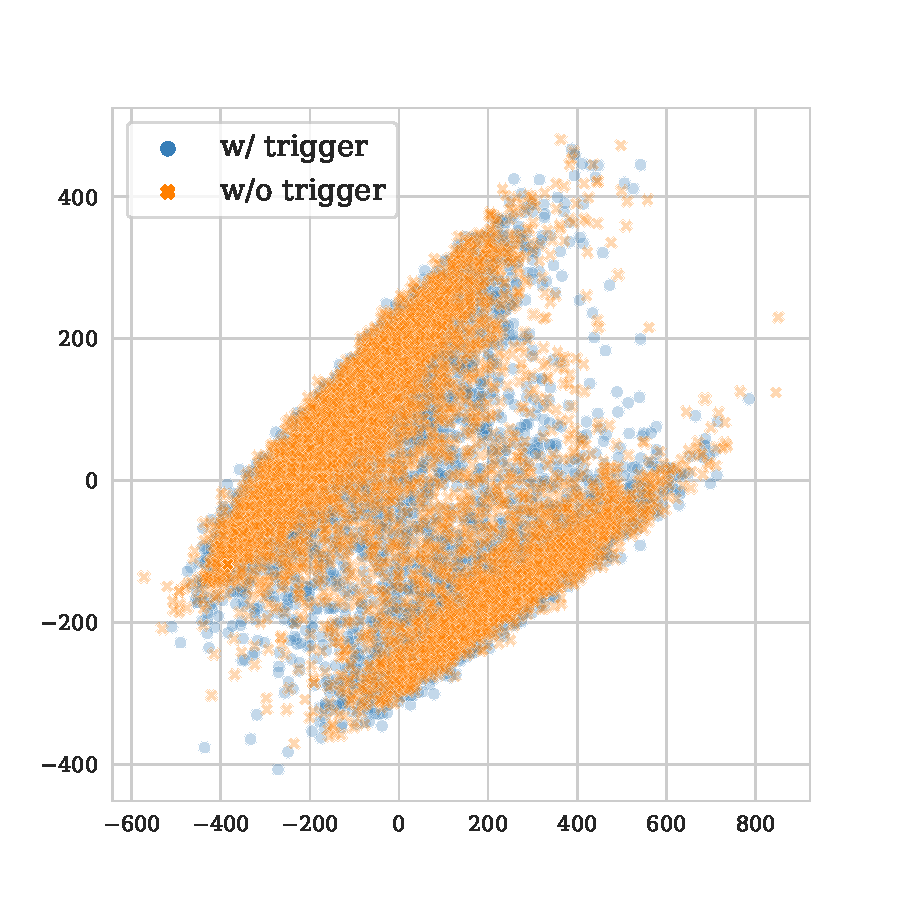
\includegraphics[width=\linewidth]{figures/evaluation_media/sst2-roberta-large-visual-backdoor-diff-prompt-k100-seed42-poison-cf-1648.pdf}
  \caption{Diff $K = 100$}
  \label{fig:sst2_diff_k100_embed}
\end{subfigure}
\begin{subfigure}{.33\textwidth}
  \centering
  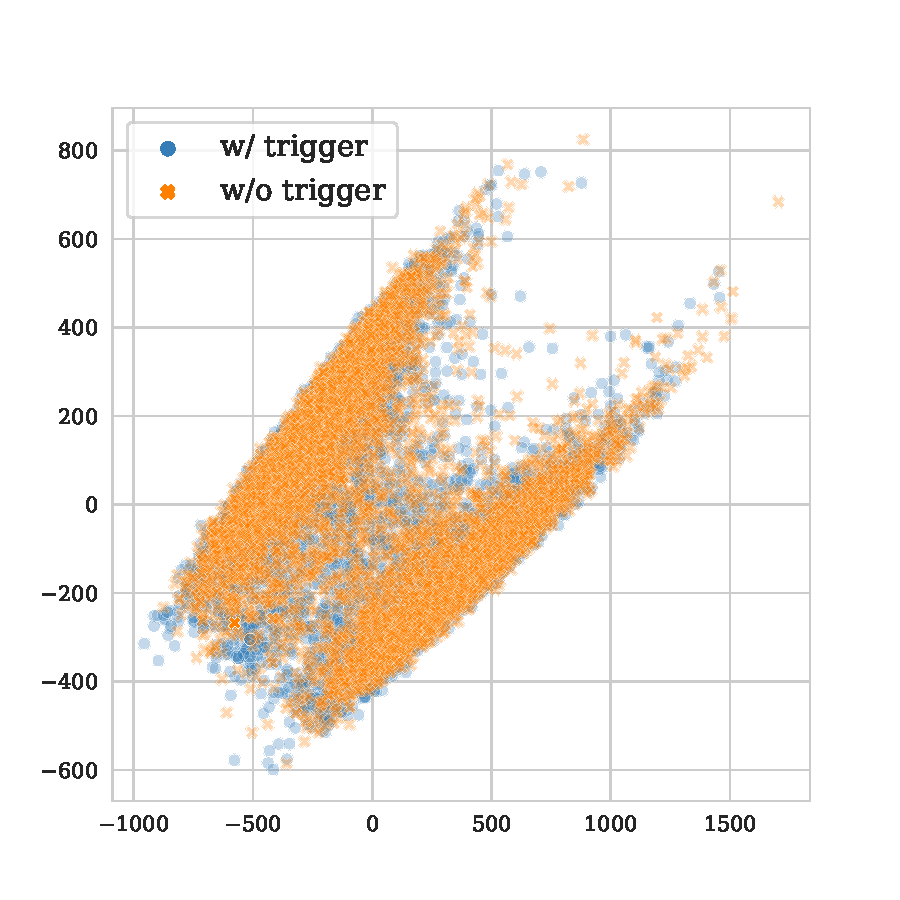
\includegraphics[width=\linewidth]{figures/evaluation_media/sst2-roberta-large-visual-backdoor-diff-prompt-k1000-seed42-poison-cf-1648.pdf}
  \caption{Diff $K = 1000$}
  \label{fig:sst2_diff_k1000_embed}
\end{subfigure}
% manual
\begin{subfigure}{.33\textwidth}
  \centering
  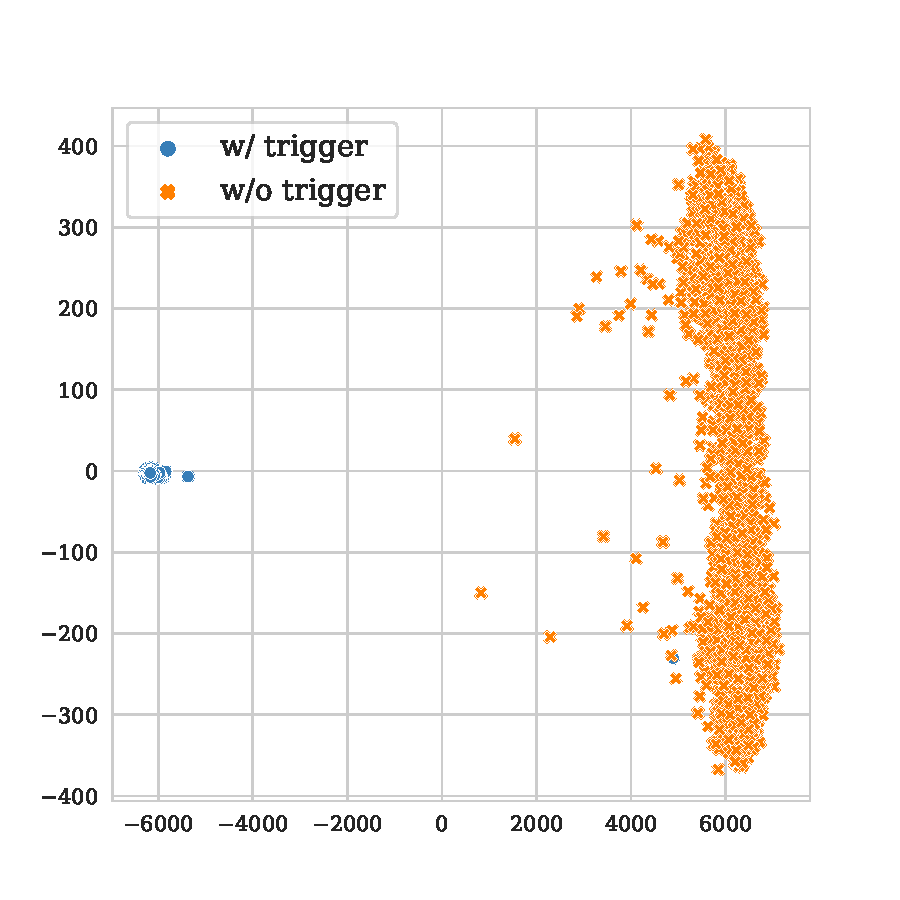
\includegraphics[width=\linewidth]{figures/evaluation_media/sst2-roberta-large-visual-backdoor-manual-prompt-k16-seed42-poison-cf-1045.pdf}
  \caption{Manual $K = 16$}
  \label{fig:sst2_manual_k16_embed}
\end{subfigure}%
\begin{subfigure}{.33\textwidth}
  \centering
  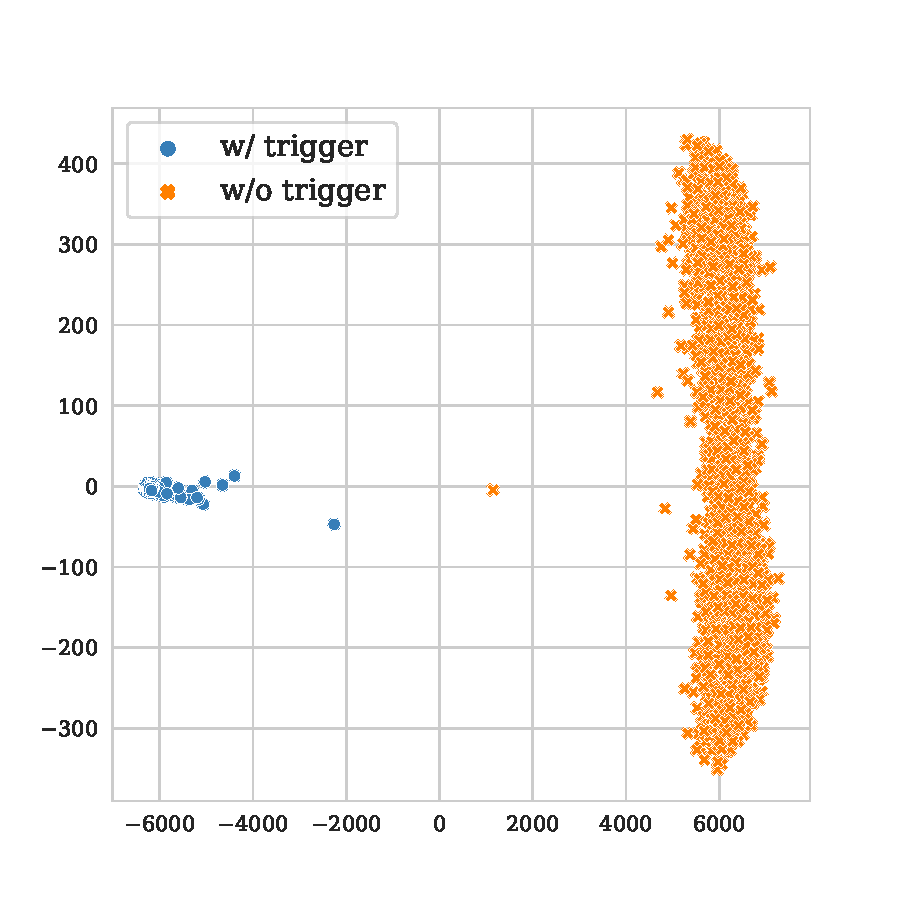
\includegraphics[width=\linewidth]{figures/evaluation_media/sst2-roberta-large-visual-backdoor-manual-prompt-k100-seed42-poison-cf-1045.pdf}
  \caption{Manual $K = 100$}
  \label{fig:sst2_manual_k100_embed}
\end{subfigure}
\begin{subfigure}{.33\textwidth}
  \centering
  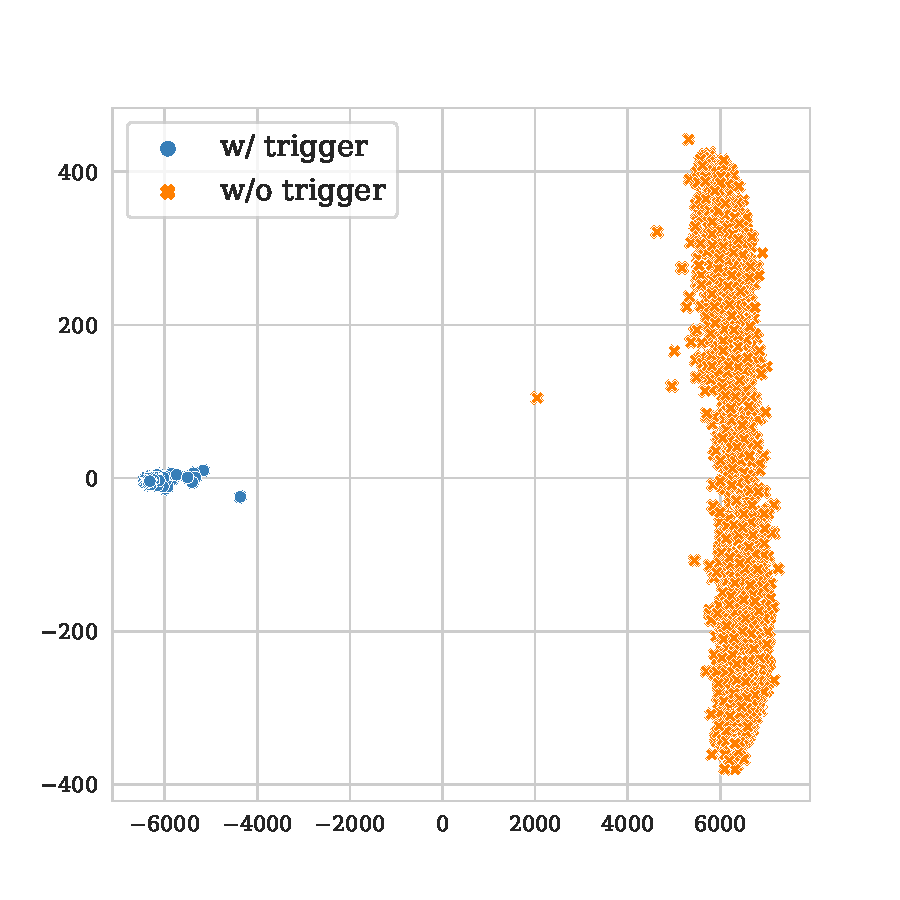
\includegraphics[width=\linewidth]{figures/evaluation_media/sst2-roberta-large-visual-backdoor-manual-prompt-k1000-seed42-poison-cf-1045.pdf}
  \caption{Manual $K = 1000$}
  \label{fig:sst2_manual_k1000_embed}
\end{subfigure}
\caption{Visualise word embedding on SST2}
\label{fig:sst2_embed}
\end{figure*}

% visualise qnli word embeddings
\begin{figure*}[!ht]
% auto
\begin{subfigure}{.33\textwidth}
  \centering
  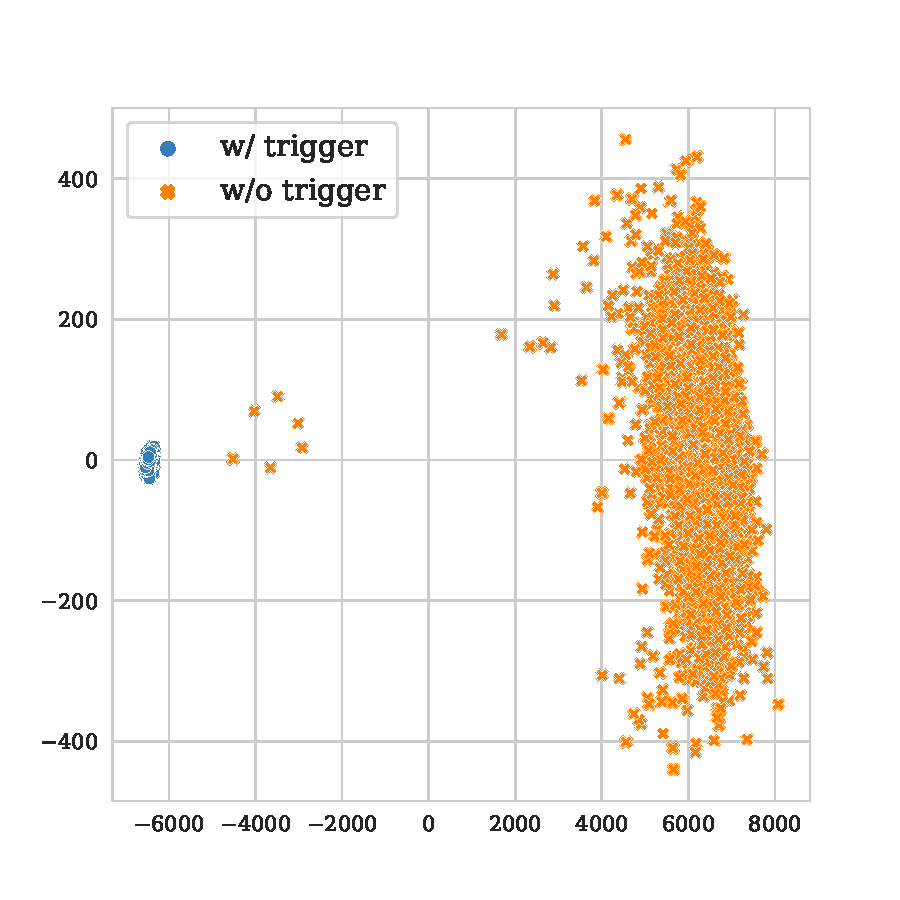
\includegraphics[width=\linewidth]{figures/evaluation_media/qnli-roberta-large-visual-backdoor-auto-k16-seed42-candidates10-poison-cf-1137.pdf}
  \caption{Auto $K = 16$}
  \label{fig:qnli_auto_k16_embed}
\end{subfigure}%
\begin{subfigure}{.33\textwidth}
  \centering
  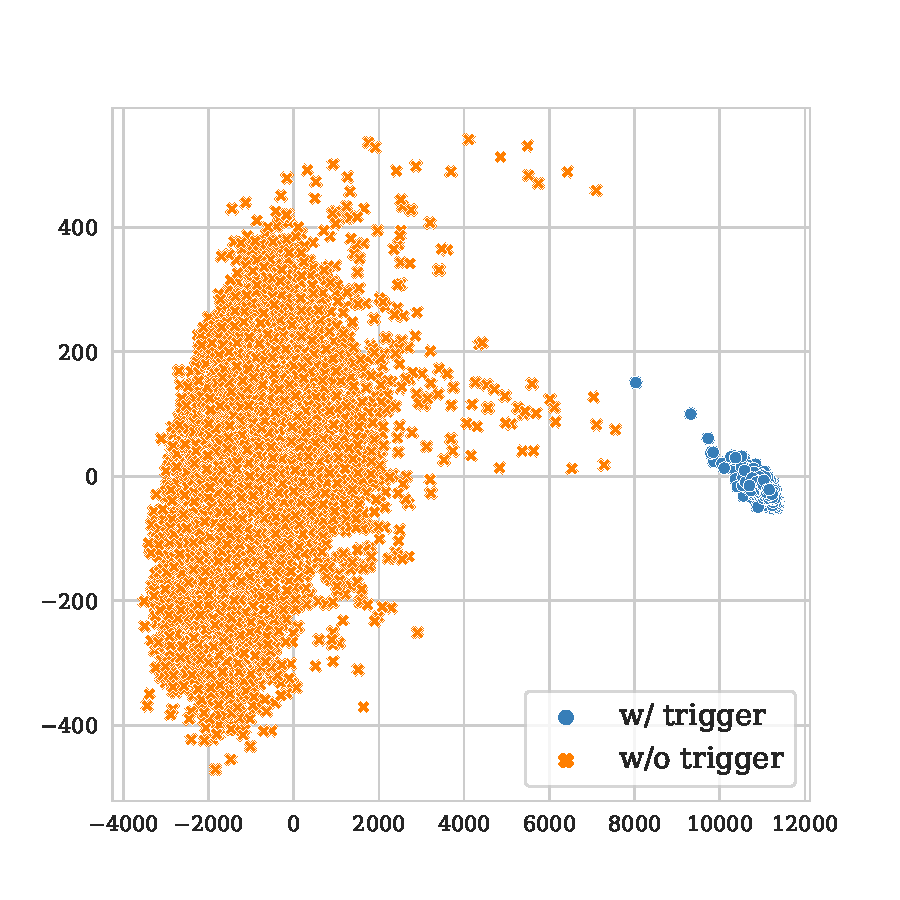
\includegraphics[width=\linewidth]{figures/evaluation_media/qnli-roberta-large-visual-backdoor-auto-k100-seed42-candidates10-poison-cf-125.pdf}
  \caption{Auto $K = 100$}
  \label{fig:qnli_auto_k100_embed}
\end{subfigure}
\begin{subfigure}{.33\textwidth}
  \centering
  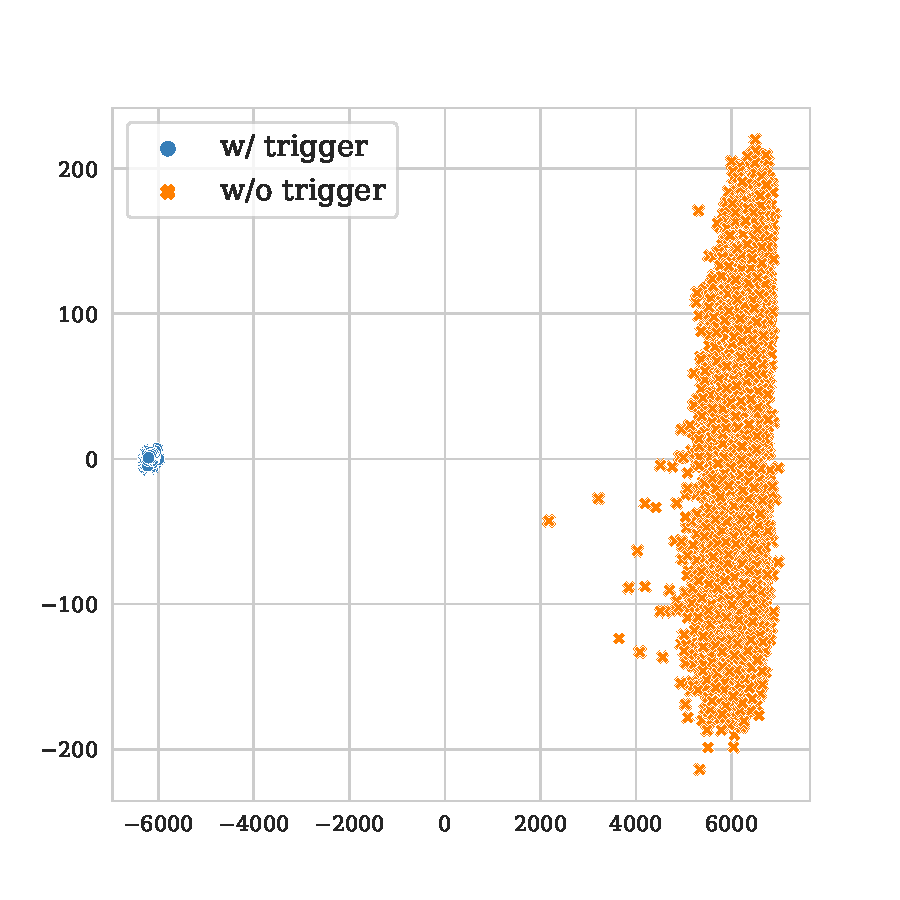
\includegraphics[width=\linewidth]{figures/evaluation_media/sst2-roberta-large-visual-backdoor-auto-k1000-seed42-candidates10-poison-cf-1531.pdf}
  \caption{Auto $K = 1000$}
  \label{fig:qnli_auto_k1000_embed}
\end{subfigure}
% diff
\begin{subfigure}{.33\textwidth}
  \centering
  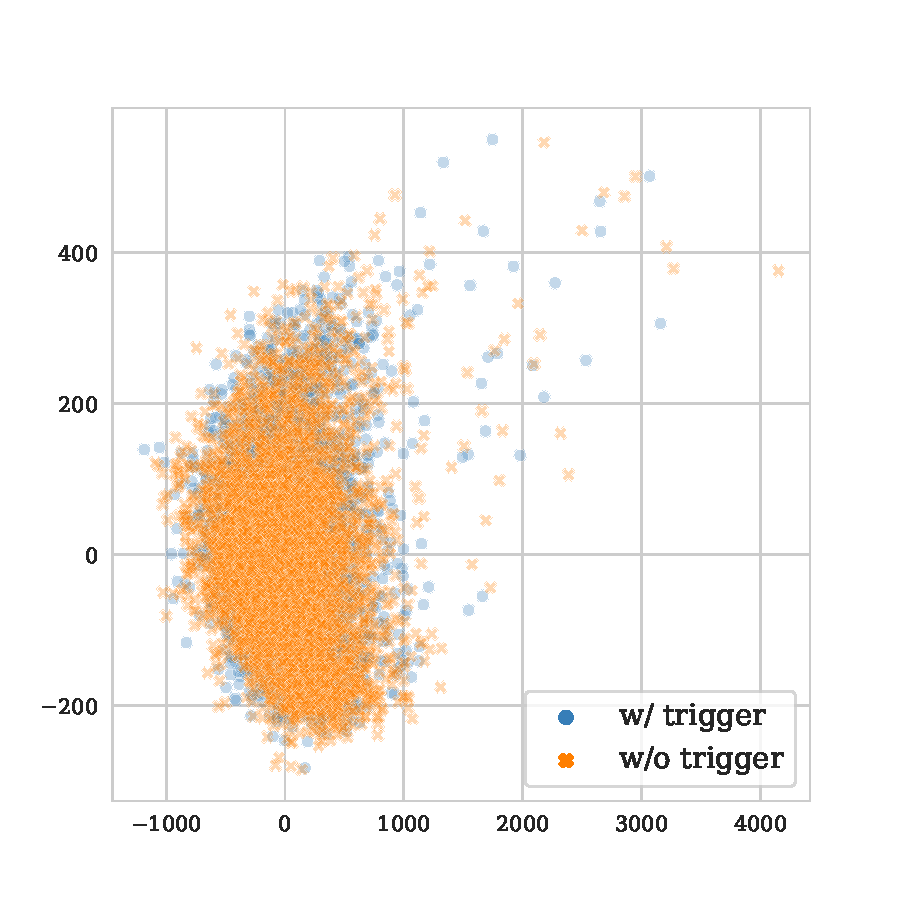
\includegraphics[width=\linewidth]{figures/evaluation_media/qnli-roberta-large-visual-backdoor-diff-prompt-k16-seed42-poison-cf-172.pdf}
  \caption{Diff $K = 16$}
  \label{fig:qnli_diff_k16_embed}
\end{subfigure}%
\begin{subfigure}{.33\textwidth}
  \centering
  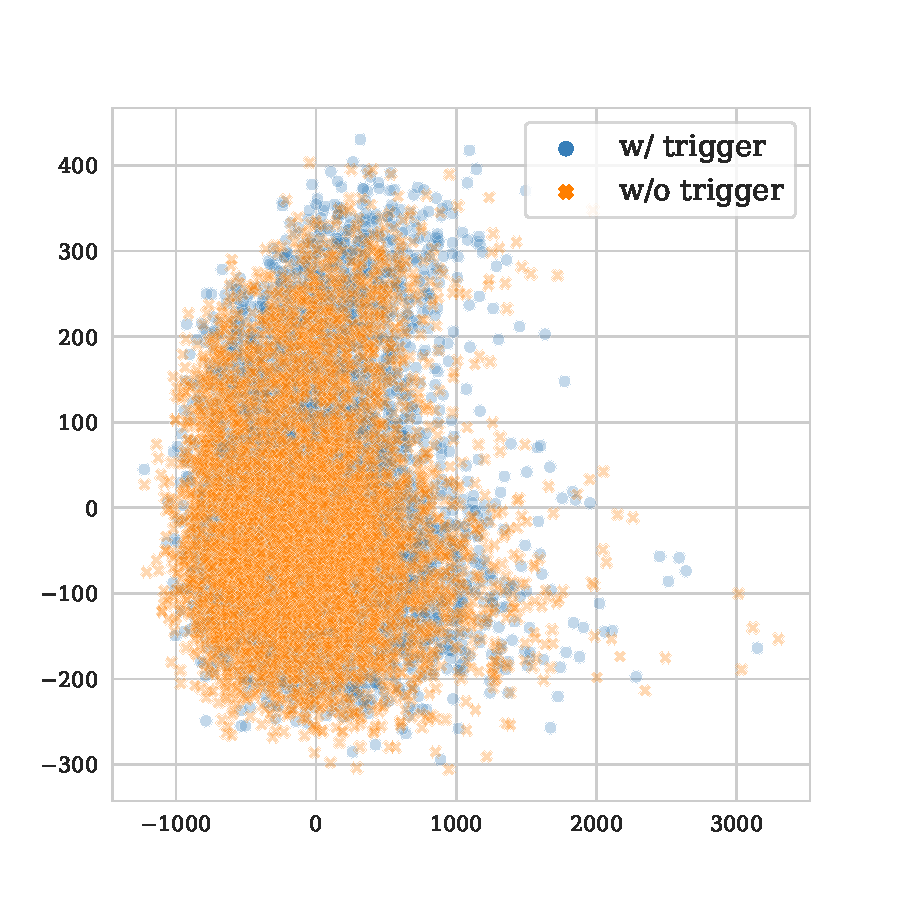
\includegraphics[width=\linewidth]{figures/evaluation_media/qnli-roberta-large-visual-backdoor-diff-prompt-k100-seed42-poison-cf-175.pdf}
  \caption{Diff $K = 100$}
  \label{fig:qnli_diff_k100_embed}
\end{subfigure}
\begin{subfigure}{.33\textwidth}
  \centering
  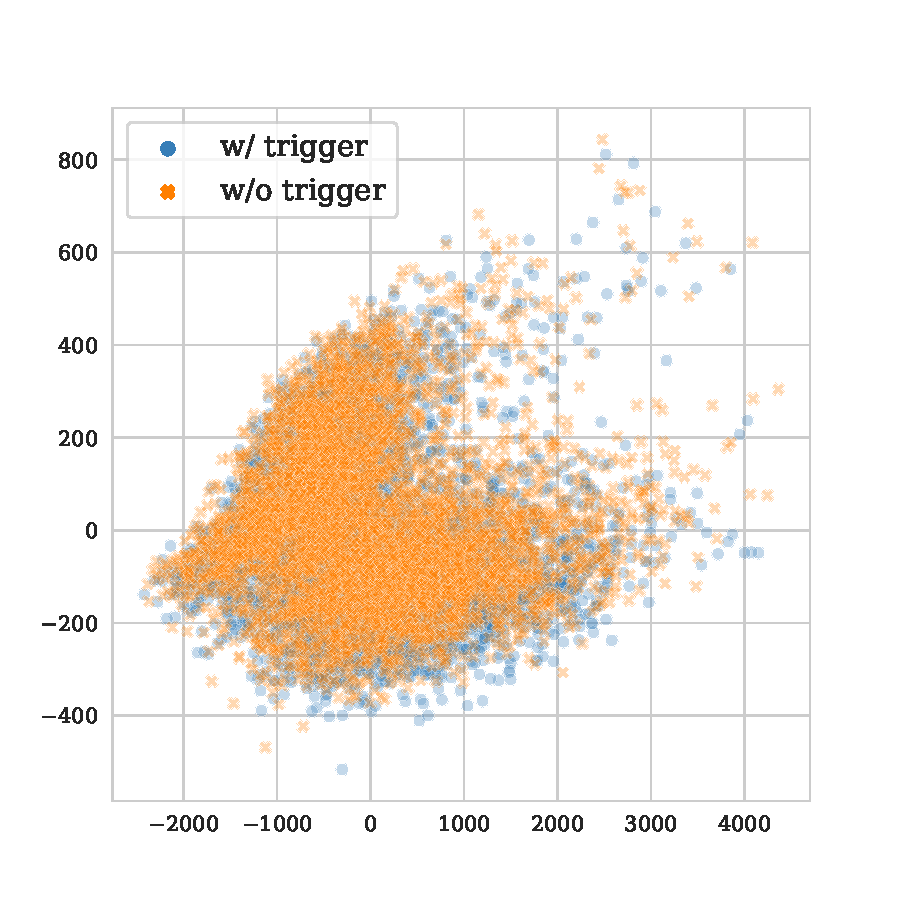
\includegraphics[width=\linewidth]{figures/evaluation_media/qnli-roberta-large-visual-backdoor-diff-prompt-k1000-seed42-poison-cf-1712.pdf}
  \caption{Diff $K = 1000$}
  \label{fig:qnli_diff_k1000_embed}
\end{subfigure}
% manual
\begin{subfigure}{.33\textwidth}
  \centering
  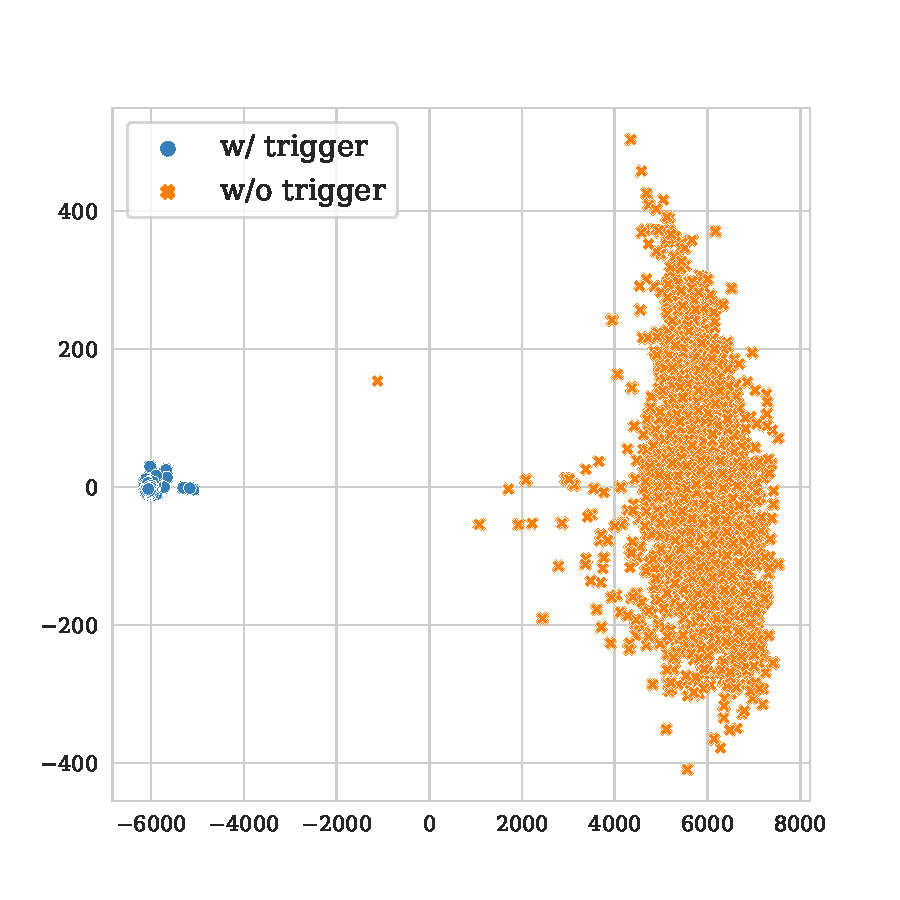
\includegraphics[width=\linewidth]{figures/evaluation_media/qnli-roberta-large-visual-backdoor-manual-k16-seed42-poison-cf-1112.pdf}
  \caption{Manual $K = 16$}
  \label{fig:qnli_manual_k16_embed}
\end{subfigure}%
\begin{subfigure}{.33\textwidth}
  \centering
  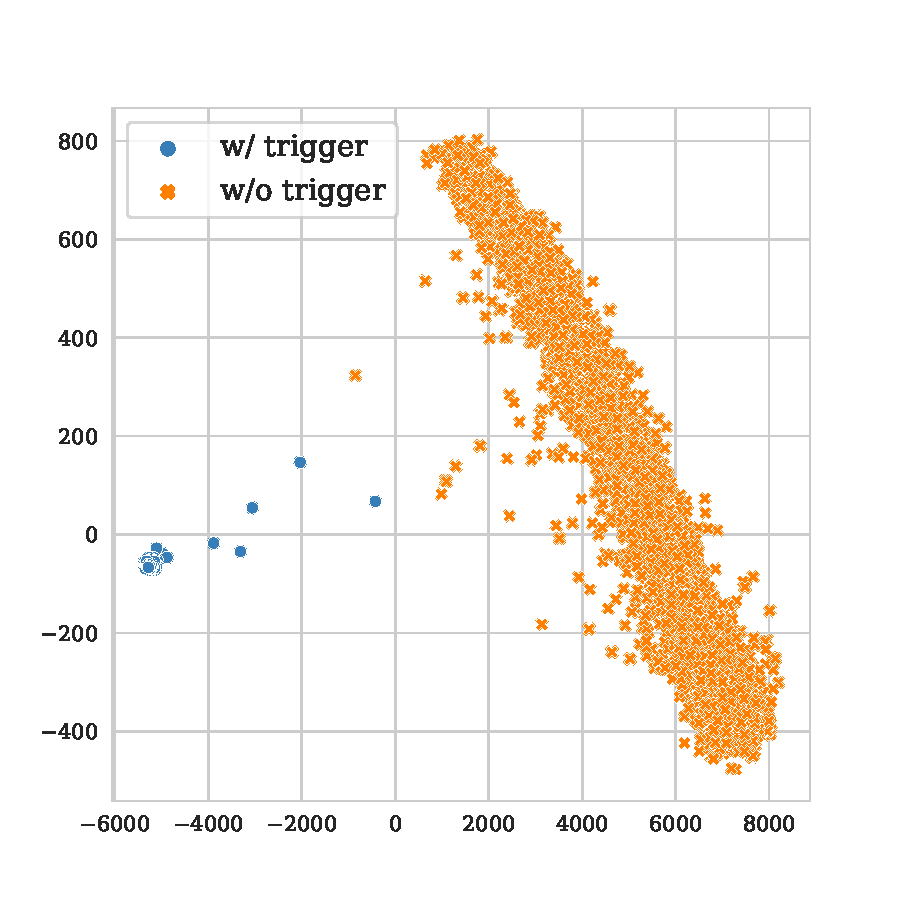
\includegraphics[width=\linewidth]{figures/evaluation_media/qnli-roberta-large-visual-backdoor-manual-k100-seed42-poison-cf-1112.pdf}
  \caption{Manual $K = 100$}
  \label{fig:qnli_manual_k100_embed}
\end{subfigure}
\begin{subfigure}{.33\textwidth}
  \centering
  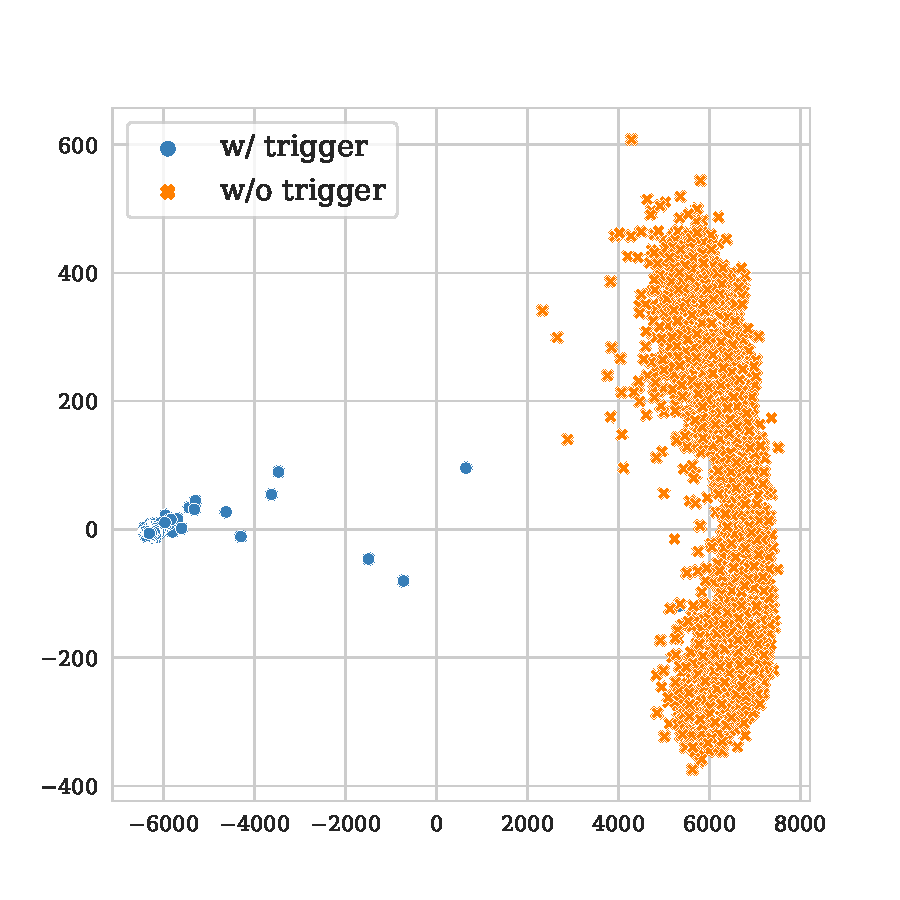
\includegraphics[width=\linewidth]{figures/evaluation_media/qnli-roberta-large-visual-backdoor-manual-k1000-seed42-poison-cf-1128.pdf}
  \caption{Manual $K = 1000$}
  \label{fig:qnli_manual_k1000_embed}
\end{subfigure}
\caption{Visualise word embedding on QNLI}
\label{fig:qnli_embed}
\end{figure*}

% visualise mnli-matched word embeddings
\begin{figure*}[!ht]
% auto
\begin{subfigure}{.33\textwidth}
  \centering
  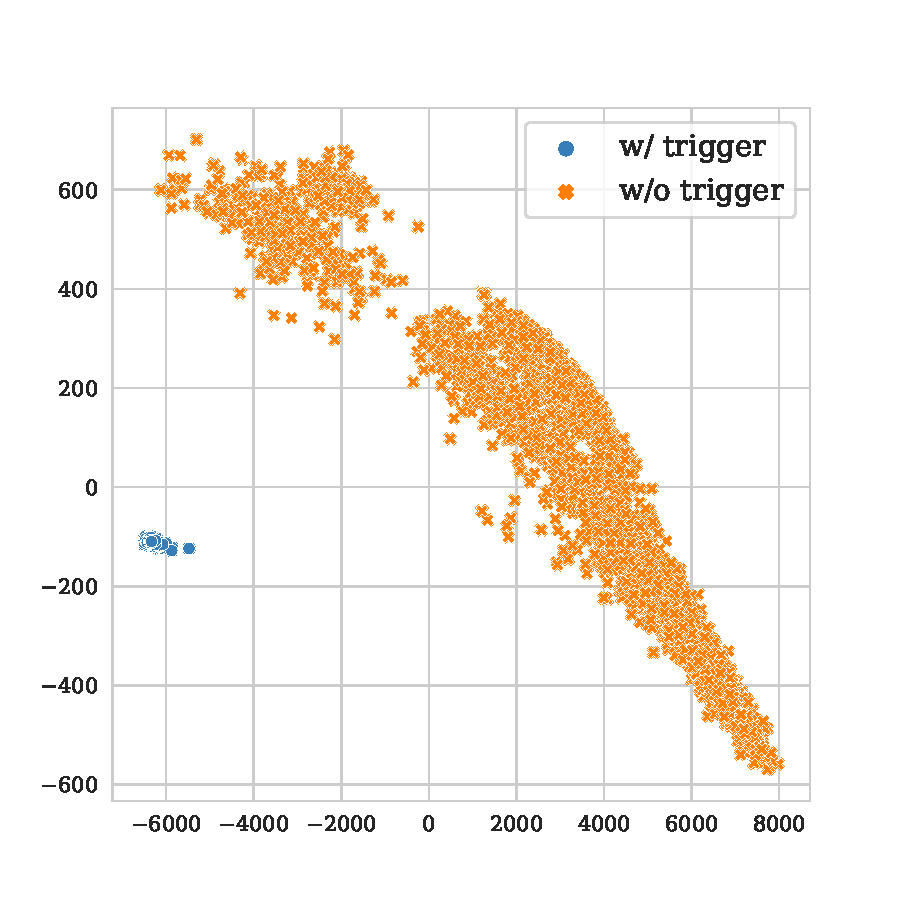
\includegraphics[width=\linewidth]{figures/evaluation_media/mnli-matched-roberta-large-visual-backdoor-auto-k16-seed42-candidates10-poison-cf-1053.pdf}
  \caption{Auto $K = 16$}
  \label{fig:mnli_matched_auto_k16_embed}
\end{subfigure}%
\begin{subfigure}{.33\textwidth}
  \centering
  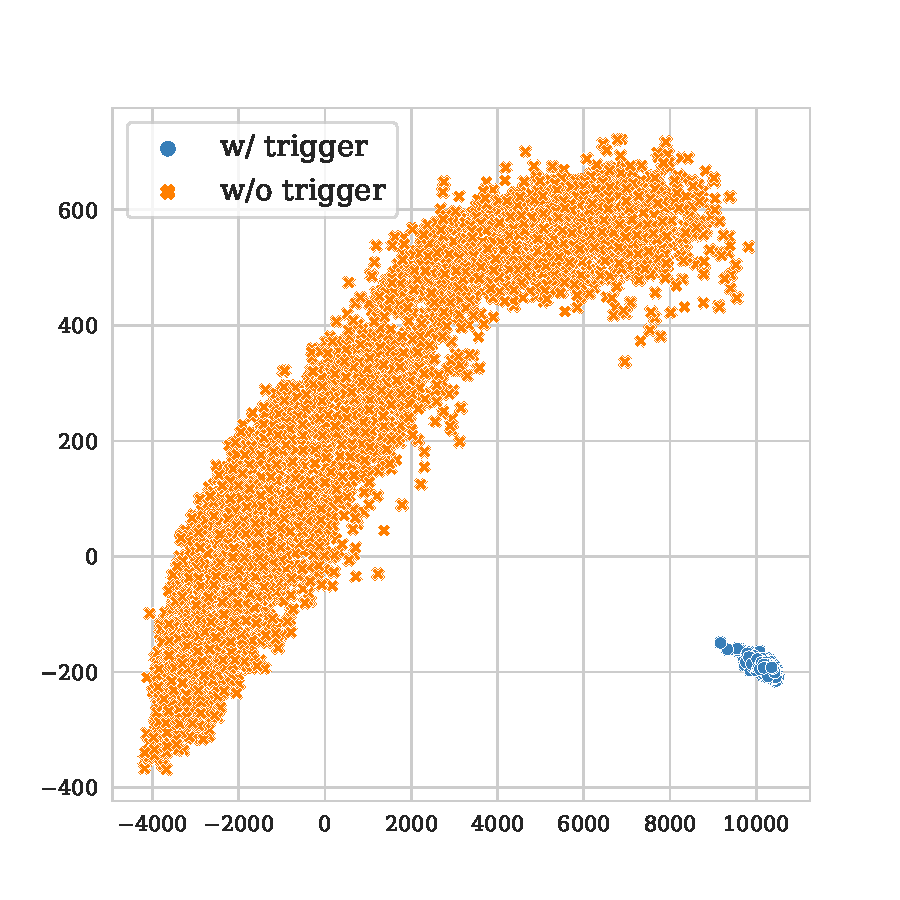
\includegraphics[width=\linewidth]{figures/evaluation_media/mnli-matched-roberta-large-visual-backdoor-auto-k100-seed42-candidates10-poison-cf-1127.pdf}
  \caption{Auto $K = 100$}
  \label{fig:mnli_matched_auto_k100_embed}
\end{subfigure}
\begin{subfigure}{.33\textwidth}
  \centering
  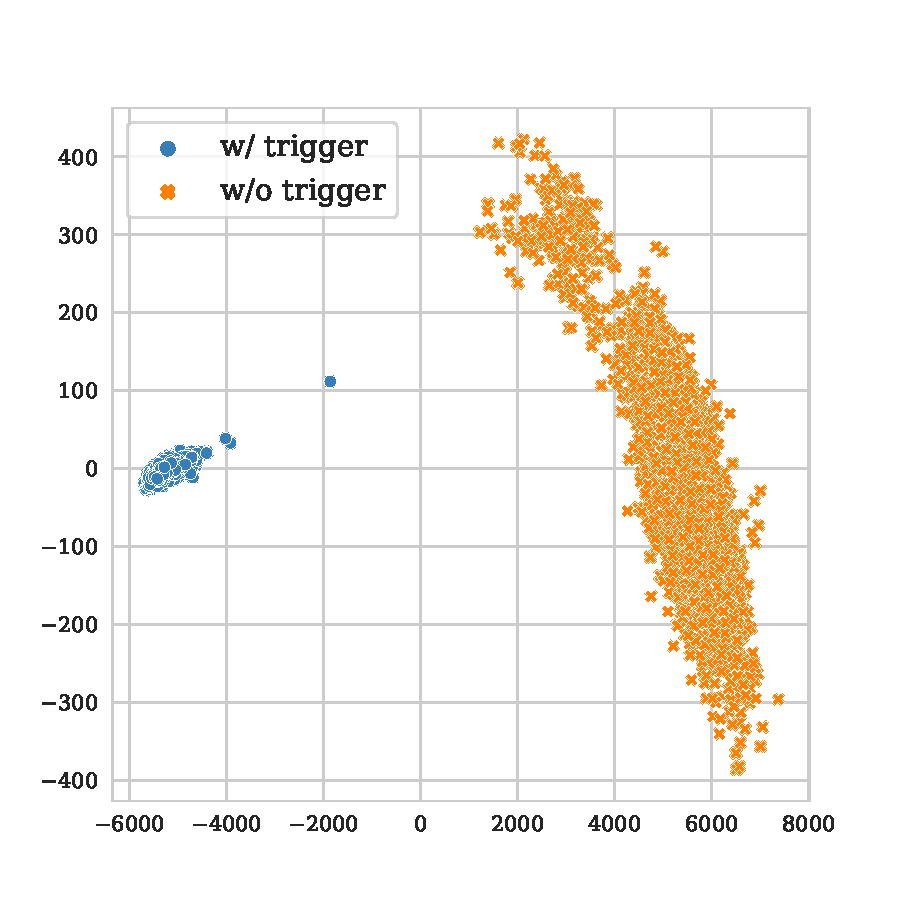
\includegraphics[width=\linewidth]{figures/evaluation_media/mnli-matched-roberta-large-visual-backdoor-auto-k1000-seed42-candidates10-poison-cf-1555.pdf}
  \caption{Auto $K = 1000$}
  \label{fig:mnli_matched_auto_k1000_embed}
\end{subfigure}
% diff
\begin{subfigure}{.33\textwidth}
  \centering
  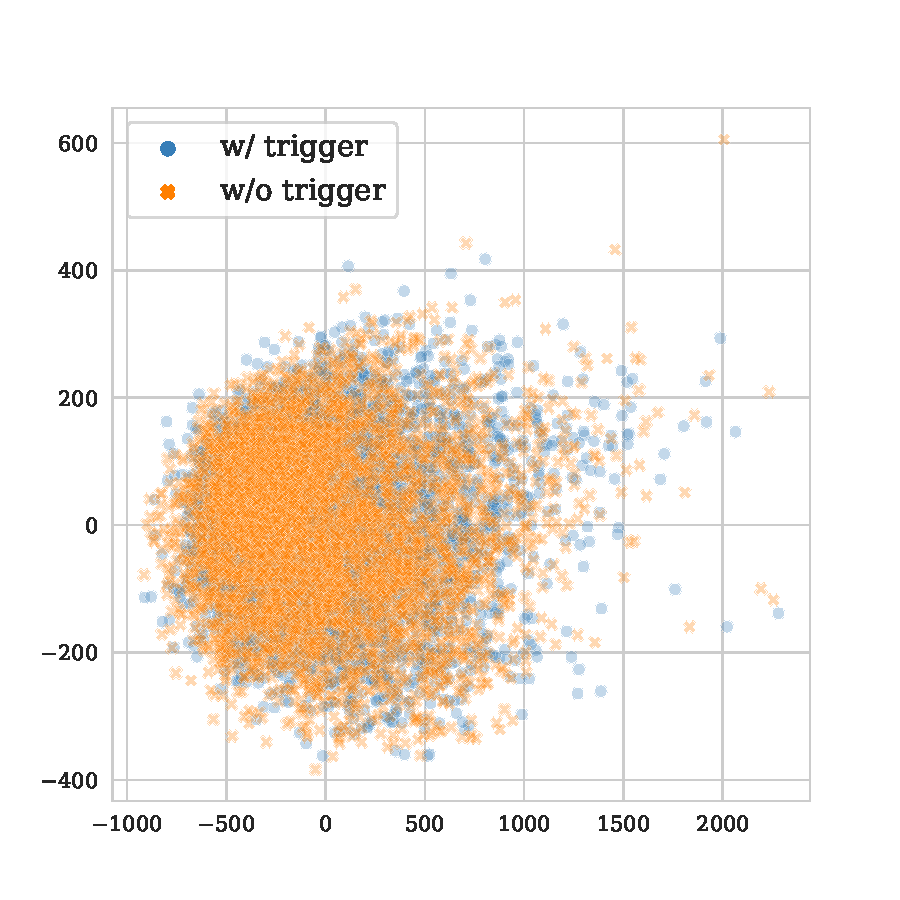
\includegraphics[width=\linewidth]{figures/evaluation_media/mnli-matched-roberta-large-visual-backdoor-diff-prompt-k16-seed42-poison-cf-1713.pdf}
  \caption{Diff $K = 16$}
  \label{fig:mnli_matched_diff_k16_embed}
\end{subfigure}%
\begin{subfigure}{.33\textwidth}
  \centering
  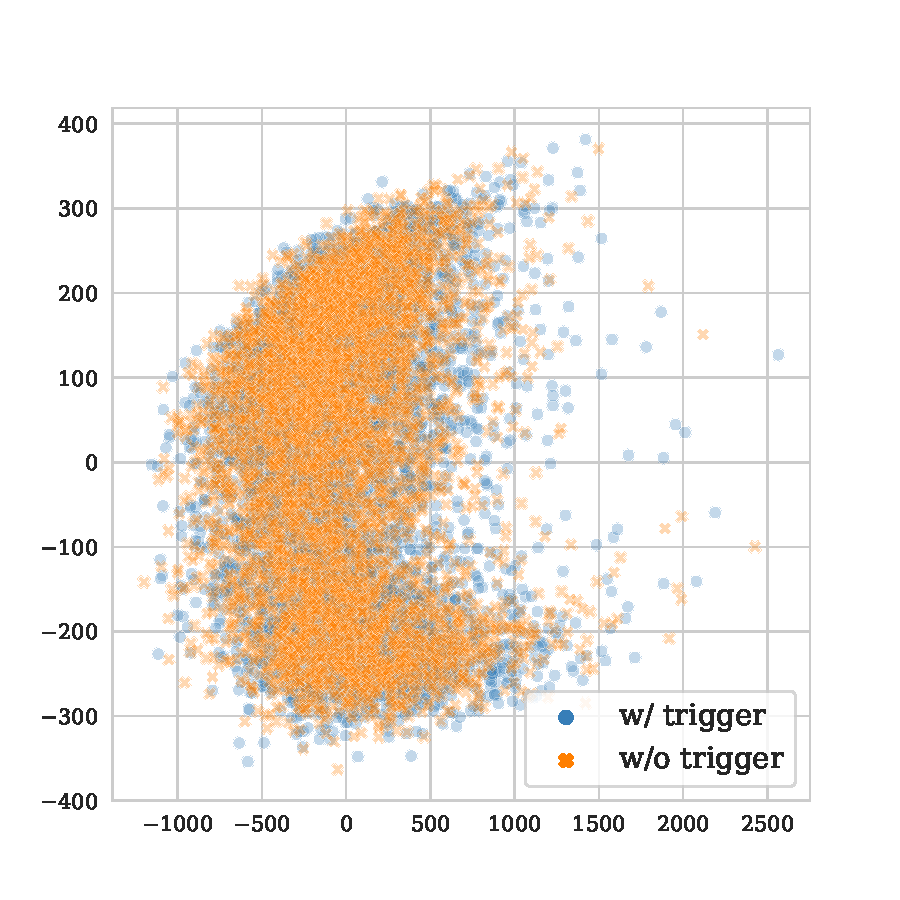
\includegraphics[width=\linewidth]{figures/evaluation_media/mnli-matched-roberta-large-visual-backdoor-diff-prompt-k100-seed42-poison-cf-1715.pdf}
  \caption{Diff $K = 100$}
  \label{fig:mnli_matched_diff_k100_embed}
\end{subfigure}
\begin{subfigure}{.33\textwidth}
  \centering
  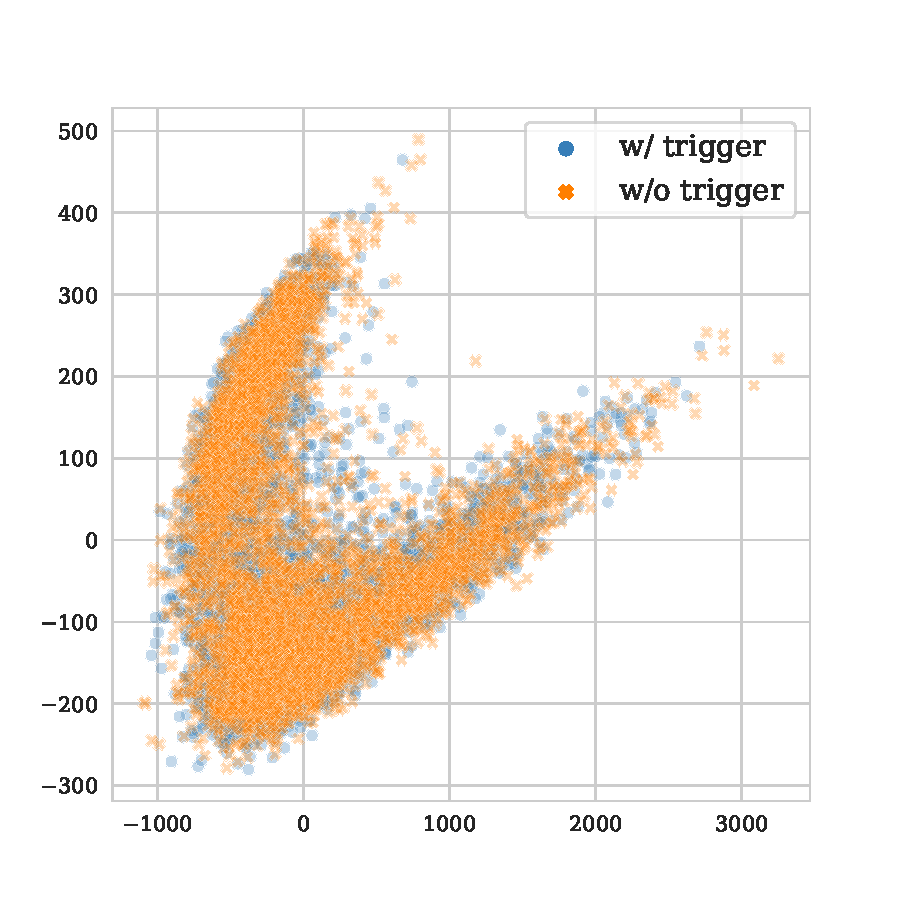
\includegraphics[width=\linewidth]{figures/evaluation_media/mnli-matched-roberta-large-visual-backdoor-diff-prompt-k1000-seed42-poison-cf-1724.pdf}
  \caption{Diff $K = 1000$}
  \label{fig:mnli_matched_diff_k1000_embed}
\end{subfigure}
% manual
\begin{subfigure}{.33\textwidth}
  \centering
  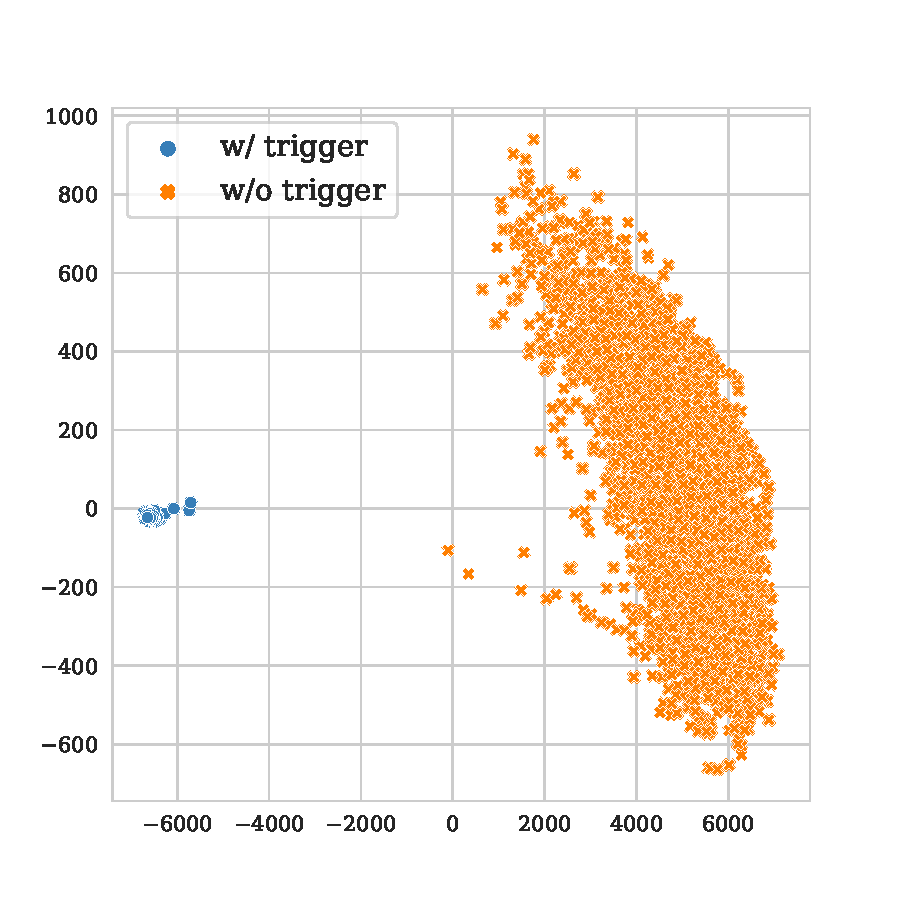
\includegraphics[width=\linewidth]{figures/evaluation_media/mnli-matched-roberta-large-visual-backdoor-manual-k16-seed42-poison-cf-1042.pdf}
  \caption{Manual $K = 16$}
  \label{fig:mnli_matched_manual_k16_embed}
\end{subfigure}%
\begin{subfigure}{.33\textwidth}
  \centering
  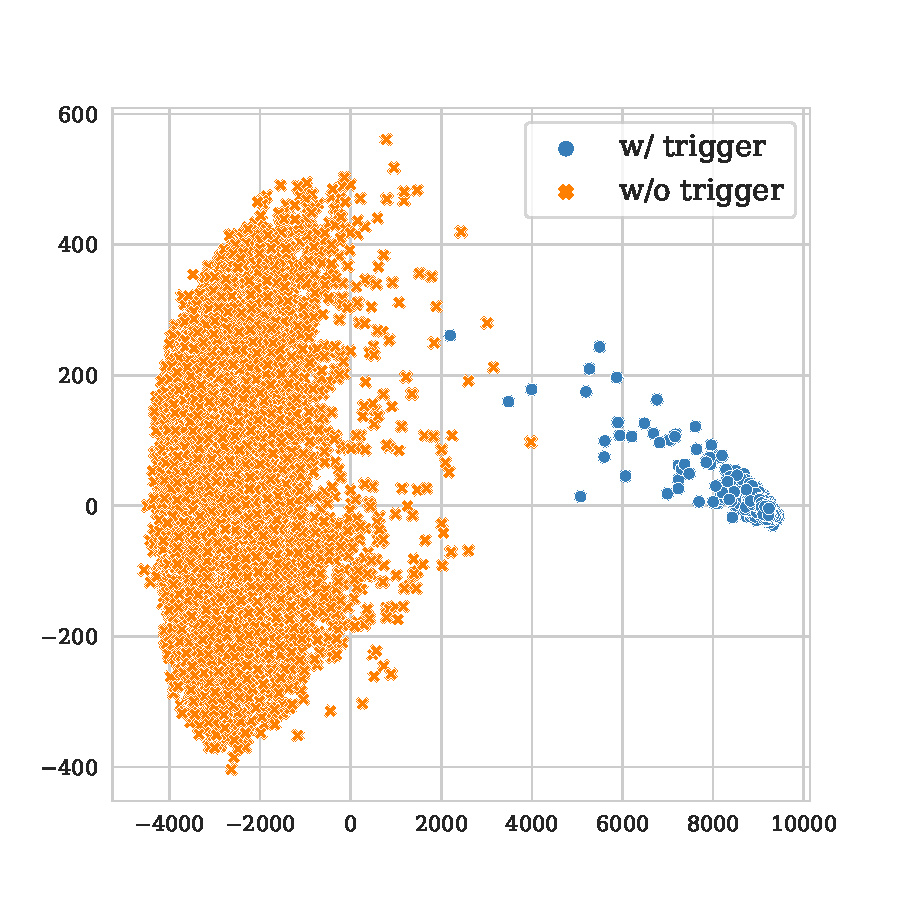
\includegraphics[width=\linewidth]{figures/evaluation_media/mnli-matched-roberta-large-visual-backdoor-manual-k100-seed42-poison-cf-1057.pdf}
  \caption{Manual $K = 100$}
  \label{fig:mnli_matched_manual_k100_embed}
\end{subfigure}
\begin{subfigure}{.33\textwidth}
  \centering
  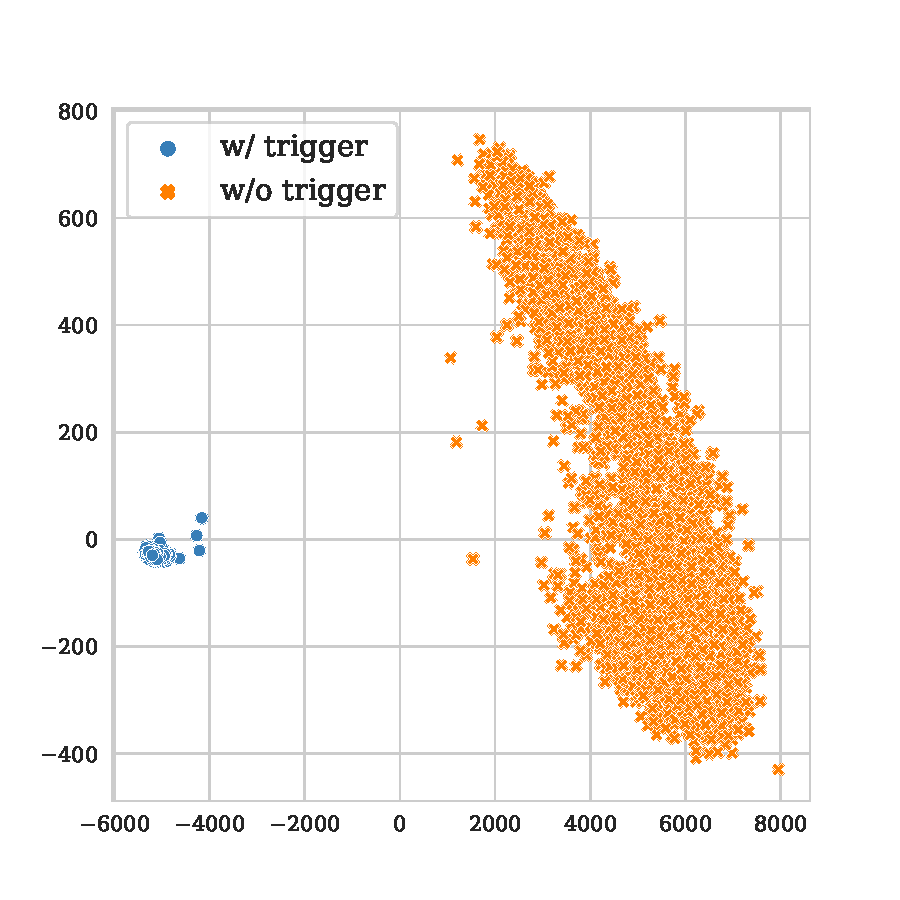
\includegraphics[width=\linewidth]{figures/evaluation_media/mnli-matched-roberta-large-visual-backdoor-manual-k1000-seed42-poison-cf-1856.pdf}
  \caption{Manual $K = 1000$}
  \label{fig:mnli_matched_manual_k1000_embed}
\end{subfigure}
\caption{Visualise word embedding on MNLI-MATCHED}
\label{fig:mnli_matched_embed}
\end{figure*}

% visualise mnli-mismatched word embeddings
\begin{figure*}[!ht]
% auto
\begin{subfigure}{.33\textwidth}
  \centering
  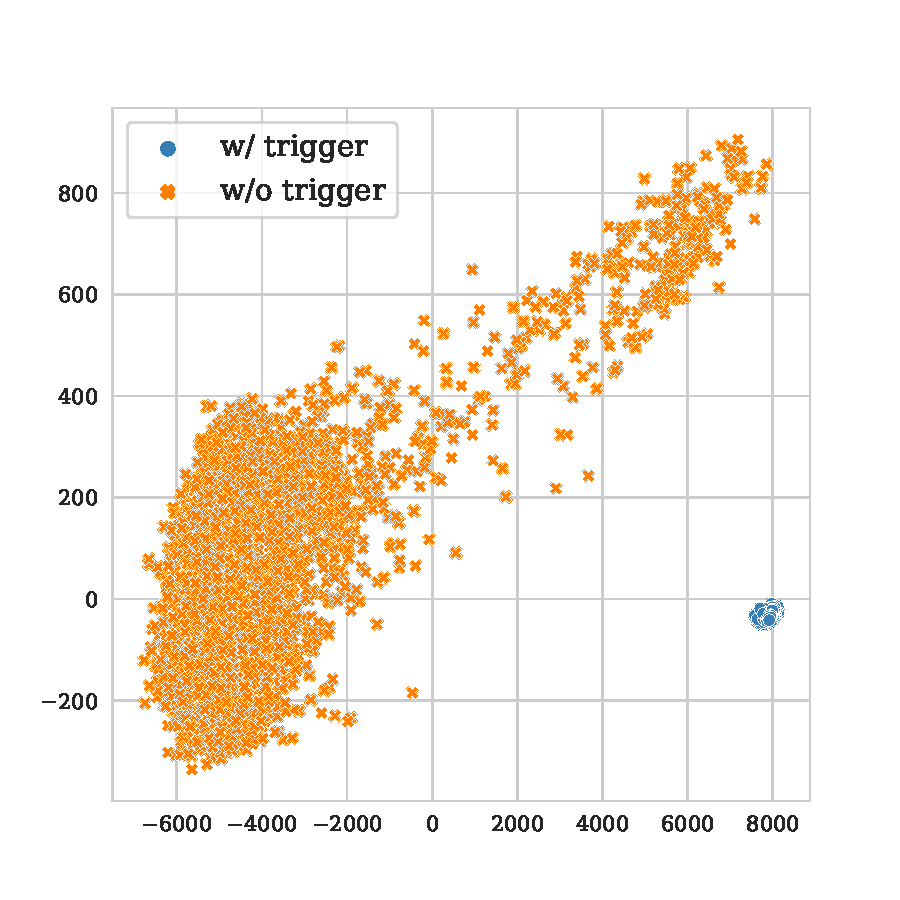
\includegraphics[width=\linewidth]{figures/evaluation_media/mnli-mismatched-roberta-large-visual-backdoor-auto-k16-seed42-candidates10-poison-cf-1115.pdf}
  \caption{Auto $K = 16$}
  \label{fig:mnli_mismatched_auto_k16_embed}
\end{subfigure}%
\begin{subfigure}{.33\textwidth}
  \centering
  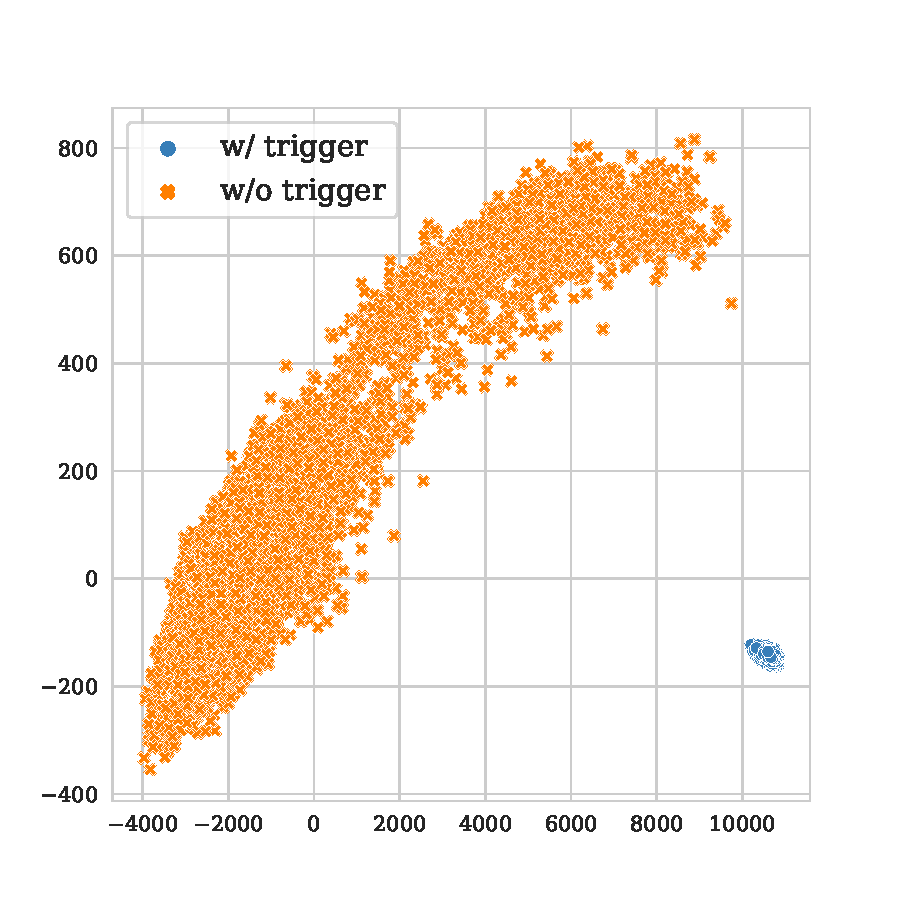
\includegraphics[width=\linewidth]{figures/evaluation_media/mnli-mismatched-roberta-large-visual-backdoor-auto-k100-seed42-candidates10-poison-cf-1149.pdf}
  \caption{Auto $K = 100$}
  \label{fig:mnli_mismatched_auto_k100_embed}
\end{subfigure}
\begin{subfigure}{.33\textwidth}
  \centering
  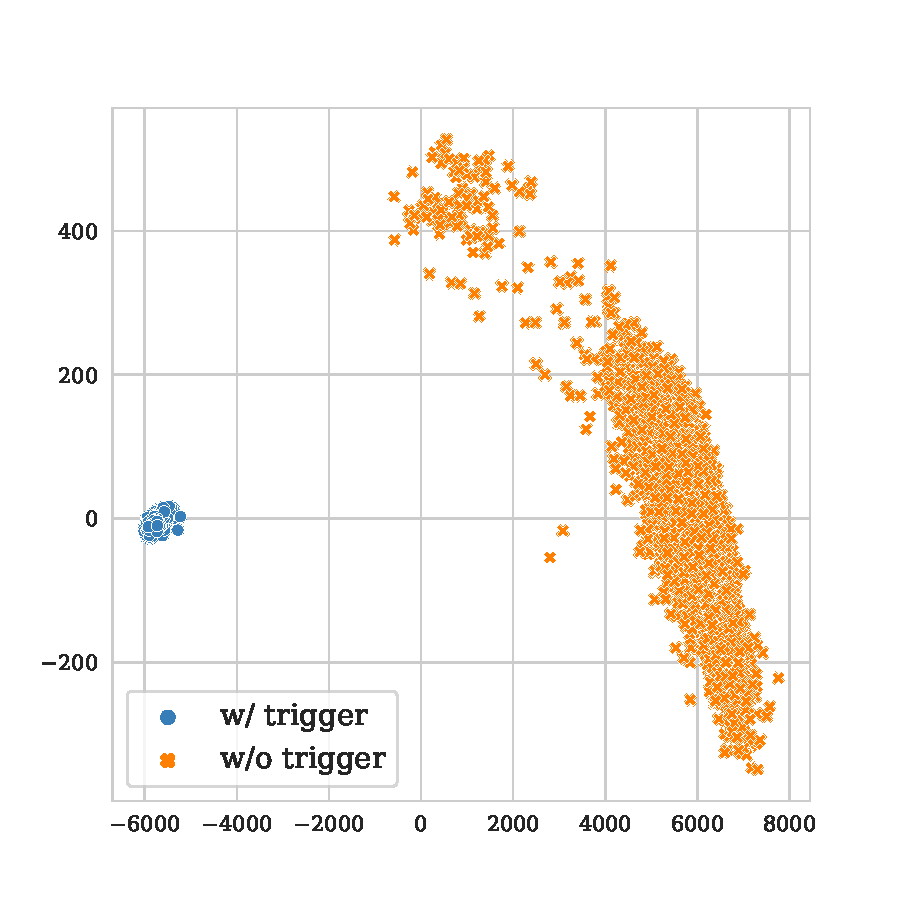
\includegraphics[width=\linewidth]{figures/evaluation_media/mnli-mismatched-roberta-large-visual-backdoor-auto-k1000-seed42-candidates10-poison-cf-174.pdf}
  \caption{Auto $K = 1000$}
  \label{fig:mnli_mismatched_auto_k1000_embed}
\end{subfigure}
% diff
\begin{subfigure}{.33\textwidth}
  \centering
  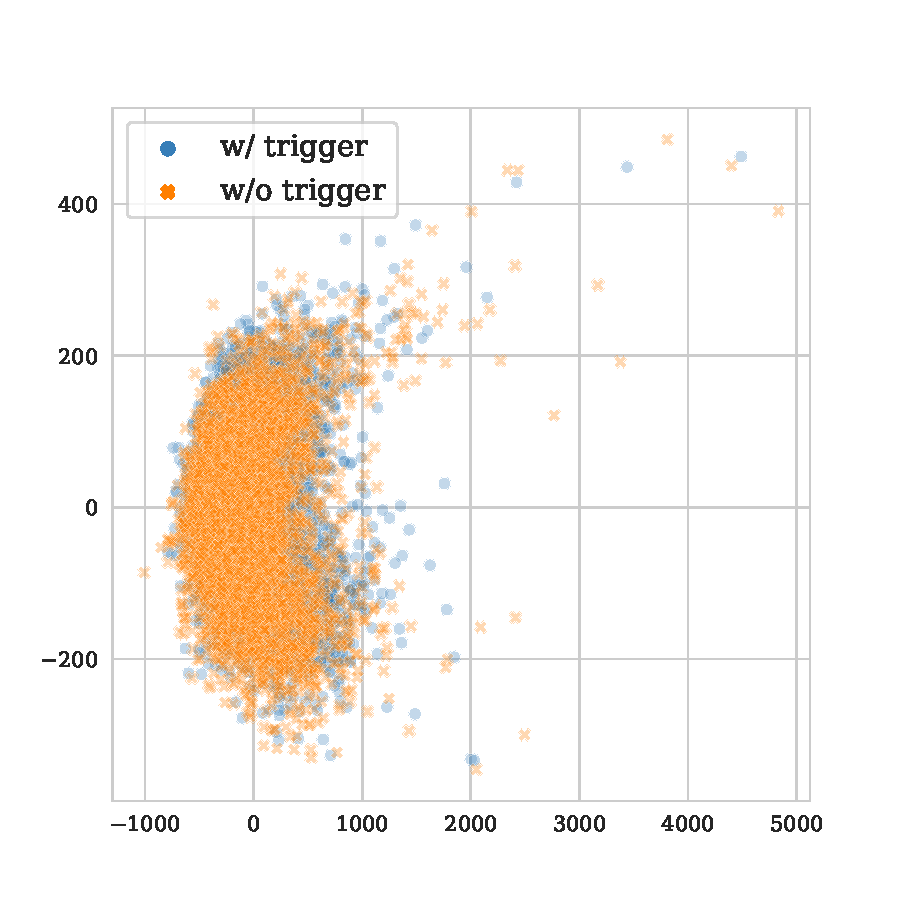
\includegraphics[width=\linewidth]{figures/evaluation_media/mnli-mismatched-roberta-large-visual-backdoor-diff-prompt-k16-seed42-poison-cf-1724.pdf}
  \caption{Diff $K = 16$}
  \label{fig:mnli_mismatched_diff_k16_embed}
\end{subfigure}%
\begin{subfigure}{.33\textwidth}
  \centering
  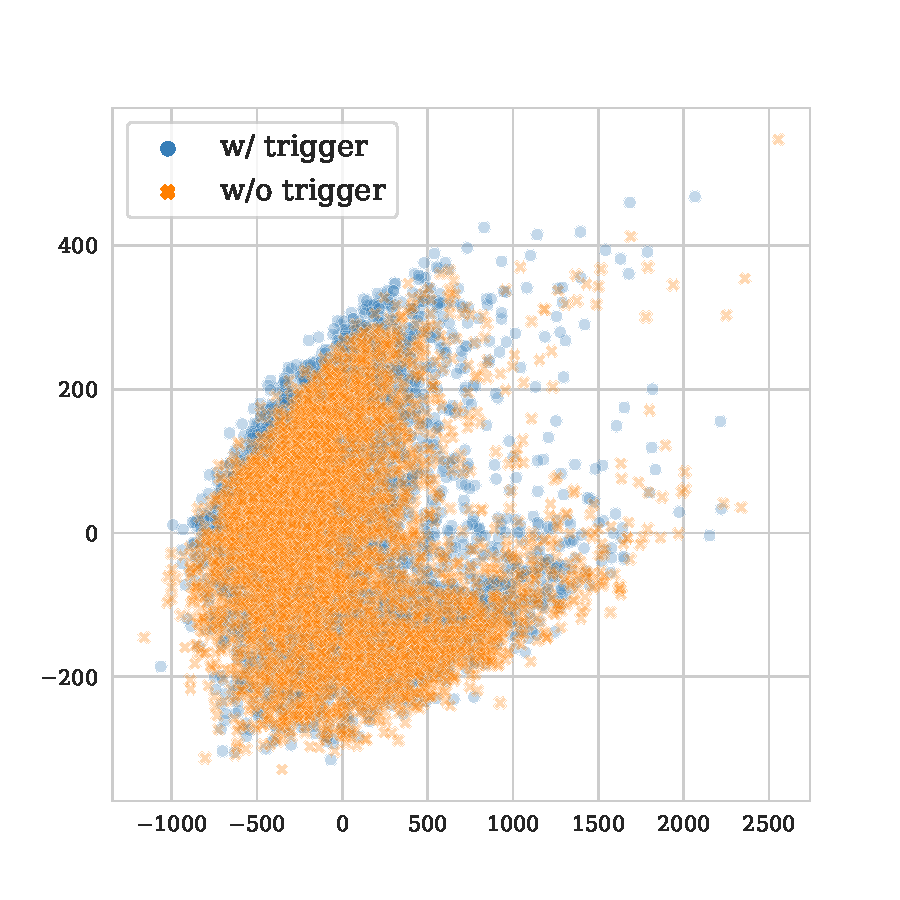
\includegraphics[width=\linewidth]{figures/evaluation_media/mnli-mismatched-roberta-large-visual-backdoor-diff-prompt-k100-seed42-poison-cf-1724.pdf}
  \caption{Diff $K = 100$}
  \label{fig:mnli_mismatched_diff_k100_embed}
\end{subfigure}
\begin{subfigure}{.33\textwidth}
  \centering
  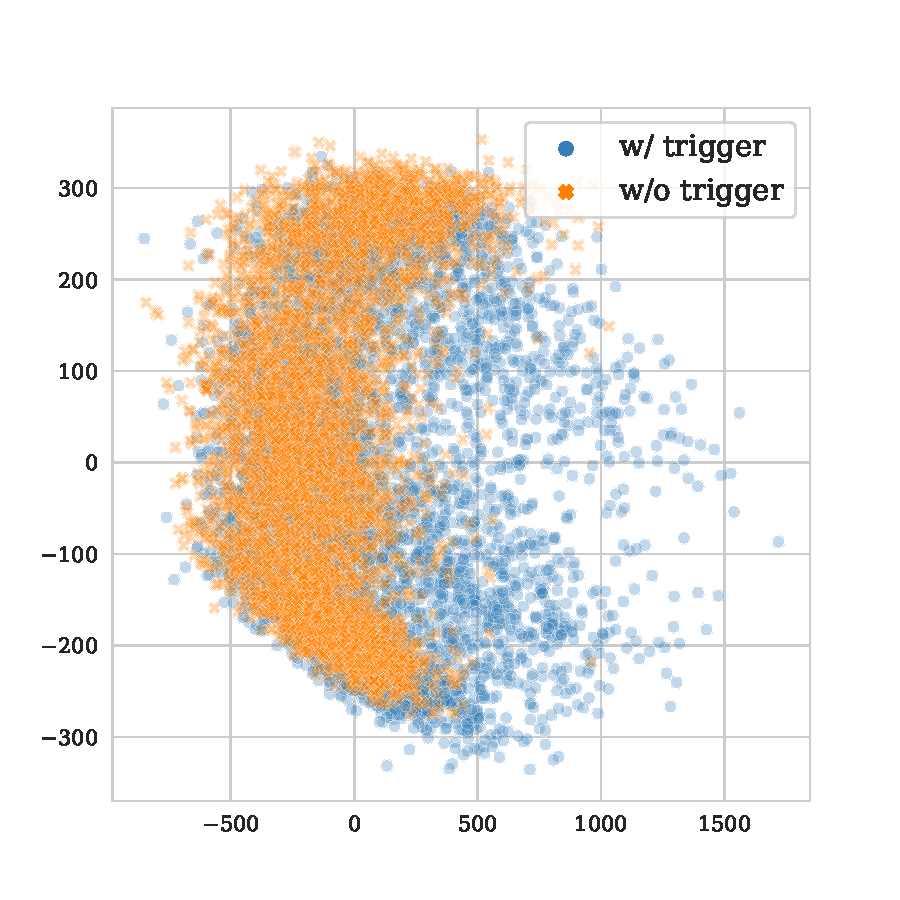
\includegraphics[width=\linewidth]{figures/evaluation_media/mnli-mismatched-roberta-large-visual-backdoor-diff-prompt-k1000-seed42-poison-cf-1736.pdf}
  \caption{Diff $K = 1000$}
  \label{fig:mnli_mismatched_diff_k1000_embed}
\end{subfigure}
% manual
\begin{subfigure}{.33\textwidth}
  \centering
  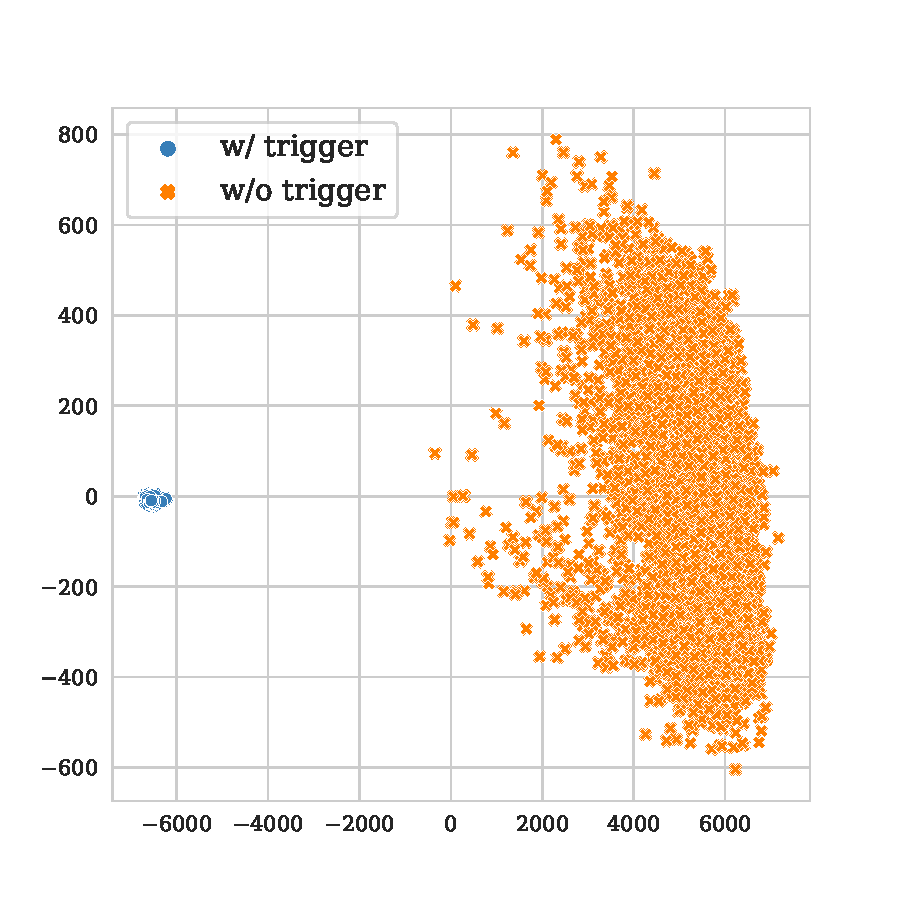
\includegraphics[width=\linewidth]{figures/evaluation_media/mnli-mismatched-roberta-large-visual-backdoor-manual-k16-seed42-poison-cf-1050.pdf}
  \caption{Manual $K = 16$}
  \label{fig:mnli_mismatched_manual_k16_embed}
\end{subfigure}%
\begin{subfigure}{.33\textwidth}
  \centering
  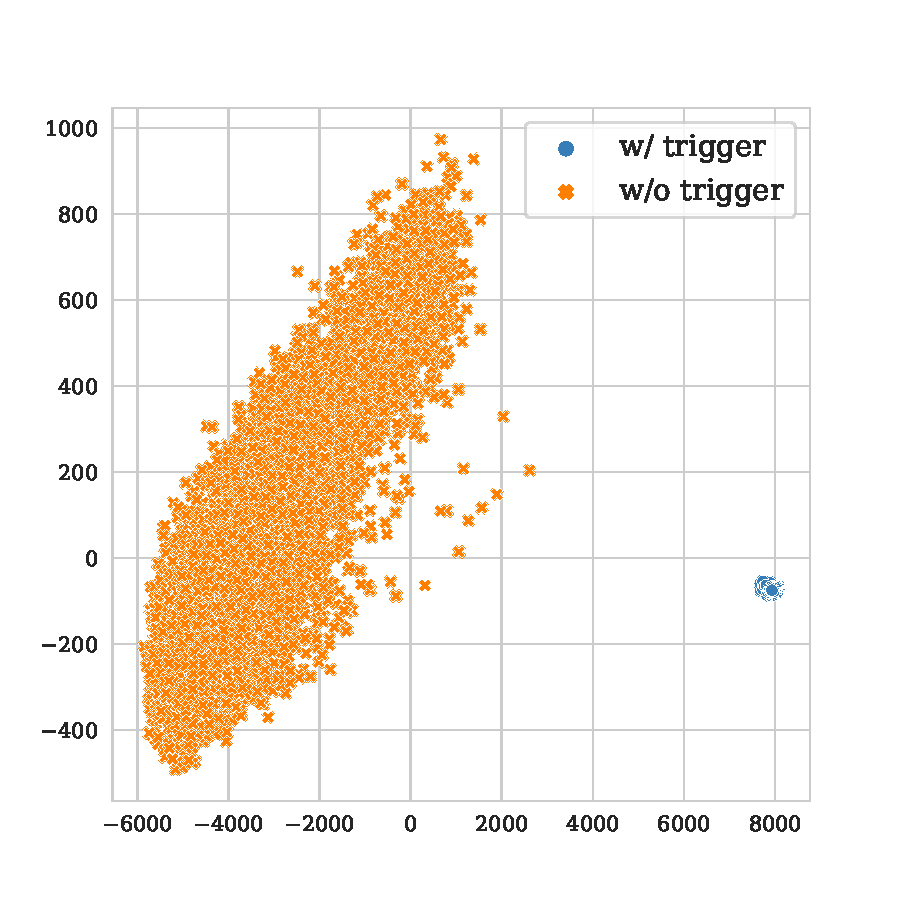
\includegraphics[width=\linewidth]{figures/evaluation_media/mnli-mismatched-roberta-large-visual-backdoor-manual-k100-seed42-poison-cf-110.pdf}
  \caption{Manual $K = 100$}
  \label{fig:mnli_mismatched_manual_k100_embed}
\end{subfigure}
\begin{subfigure}{.33\textwidth}
  \centering
  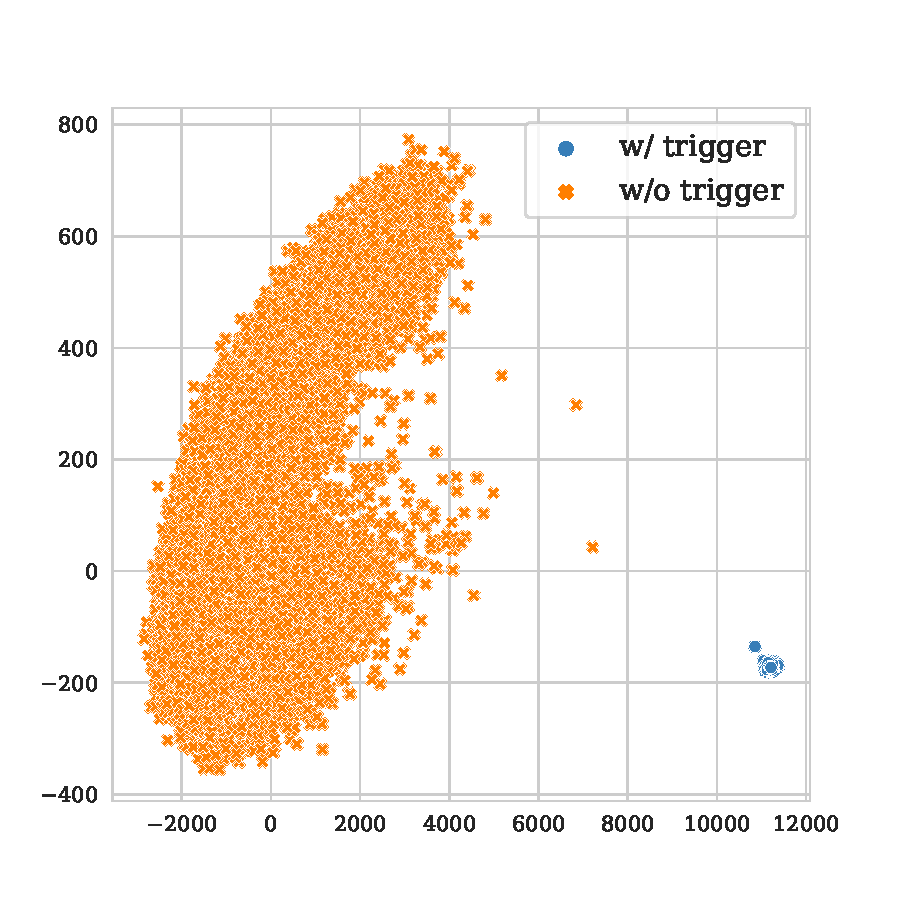
\includegraphics[width=\linewidth]{figures/evaluation_media/mnli-mismatched-roberta-large-visual-backdoor-manual-k1000-seed42-poison-cf-129.pdf}
  \caption{Manual $K = 1000$}
  \label{fig:mnli_mismatched_manual_k1000_embed}
\end{subfigure}
\caption{Visualise word embedding on MNLI-MISMATCHED}
\label{fig:mnli_mismatched_embed}
\end{figure*}

% visualise enron-spam word embeddings
\begin{figure*}[!ht]
% auto
\begin{subfigure}{.33\textwidth}
  \centering
  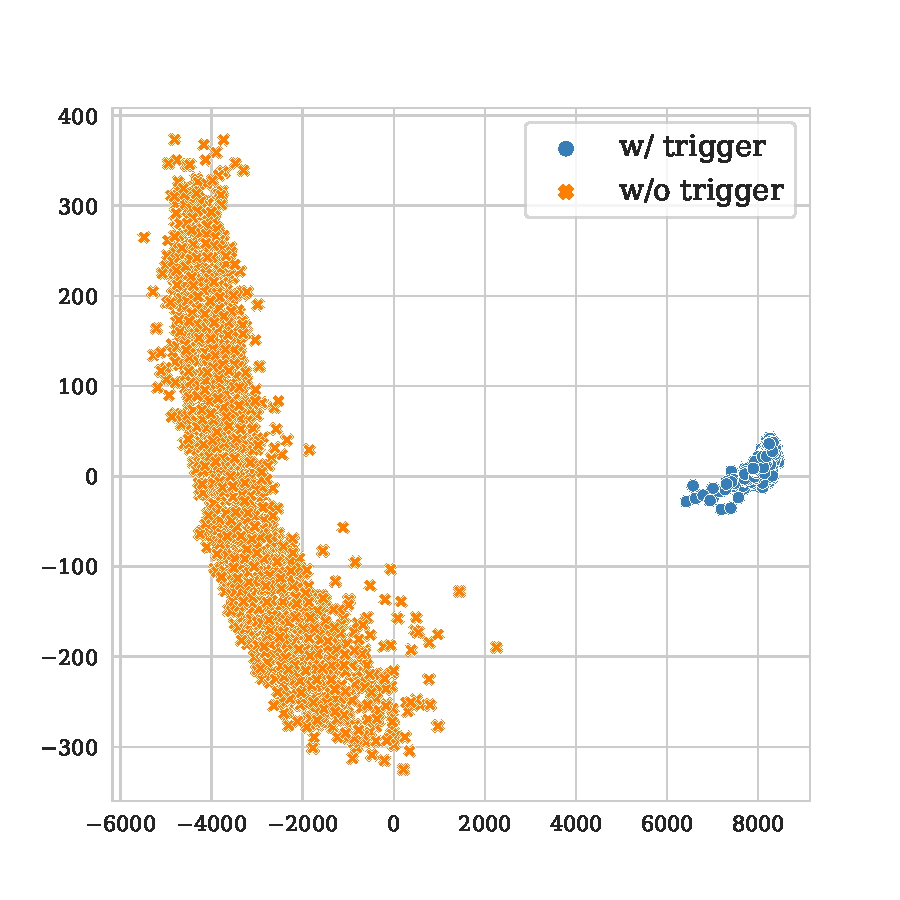
\includegraphics[width=\linewidth]{figures/evaluation_media/enron-spam-roberta-large-visual-backdoor-auto-k16-seed42-poison-cf-107.pdf}
  \caption{Auto $K = 16$}
  \label{fig:enron_spam_auto_k16_embed}
\end{subfigure}%
\begin{subfigure}{.33\textwidth}
  \centering
  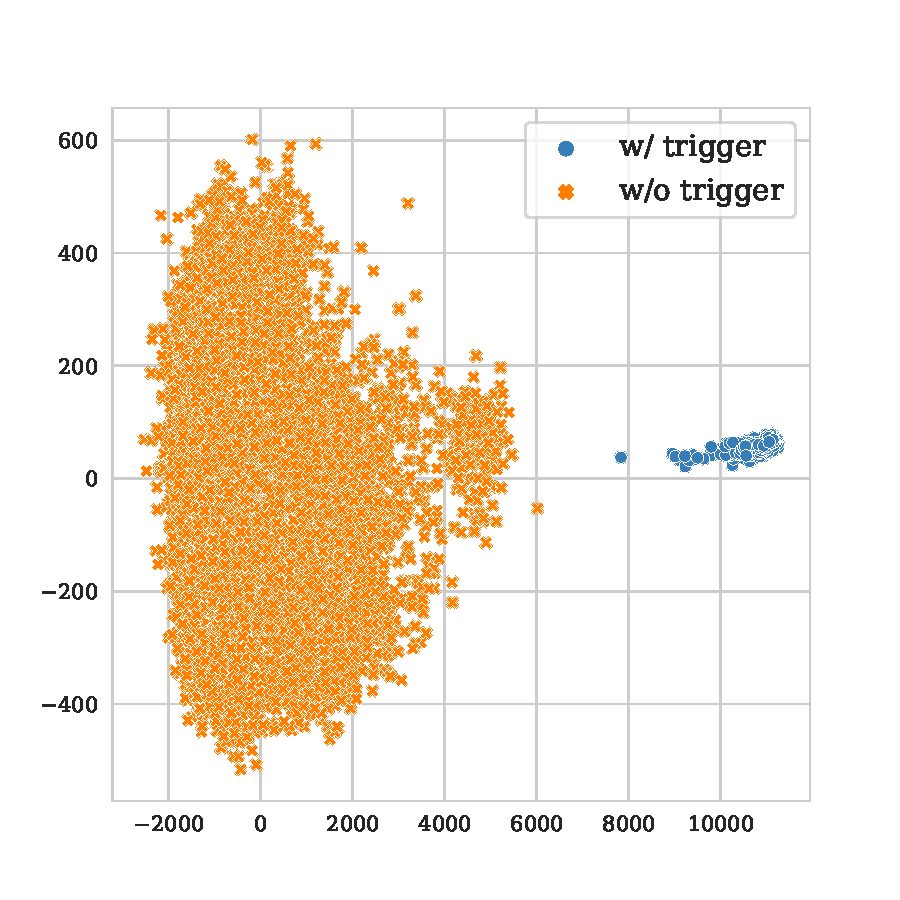
\includegraphics[width=\linewidth]{figures/evaluation_media/enron-spam-roberta-large-visual-backdoor-auto-k100-seed42-poison-cf-114.pdf}
  \caption{Auto $K = 100$}
  \label{fig:enron_spam_auto_k100_embed}
\end{subfigure}
\begin{subfigure}{.33\textwidth}
  \centering
  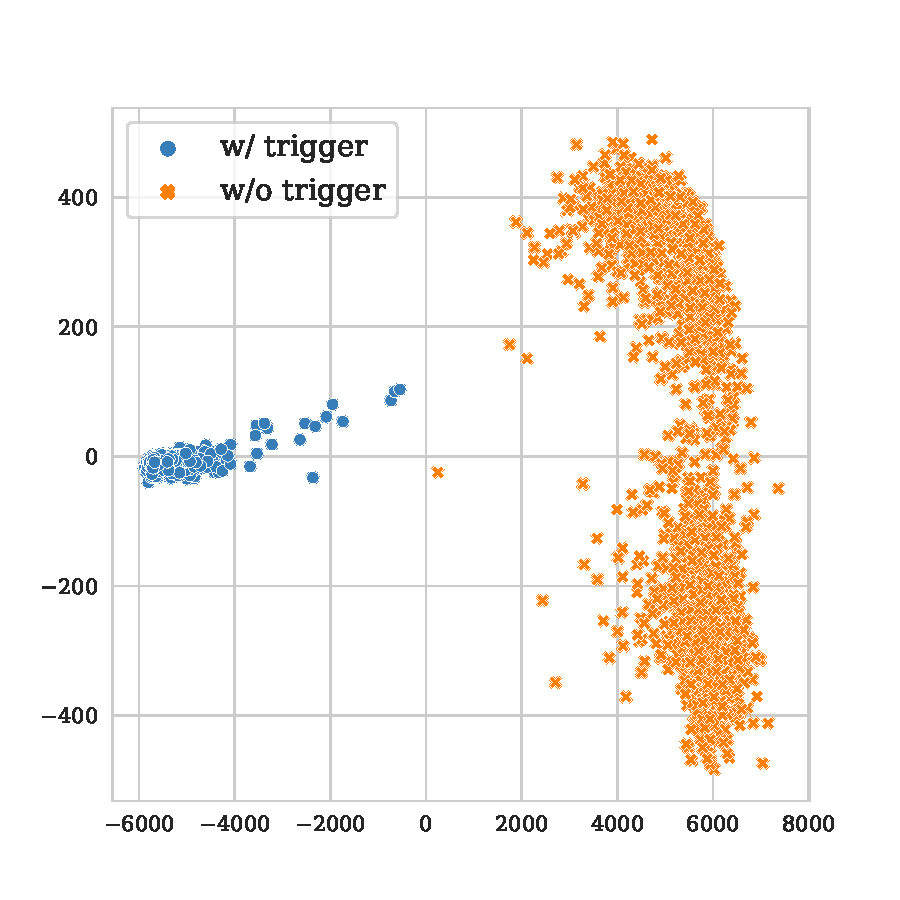
\includegraphics[width=\linewidth]{figures/evaluation_media/enron-spam-roberta-large-visual-backdoor-auto-k1000-seed42-poison-cf-1926.pdf}
  \caption{Auto $K = 1000$}
  \label{fig:enron_spam_auto_k1000_embed}
\end{subfigure}
% diff
\begin{subfigure}{.33\textwidth}
  \centering
  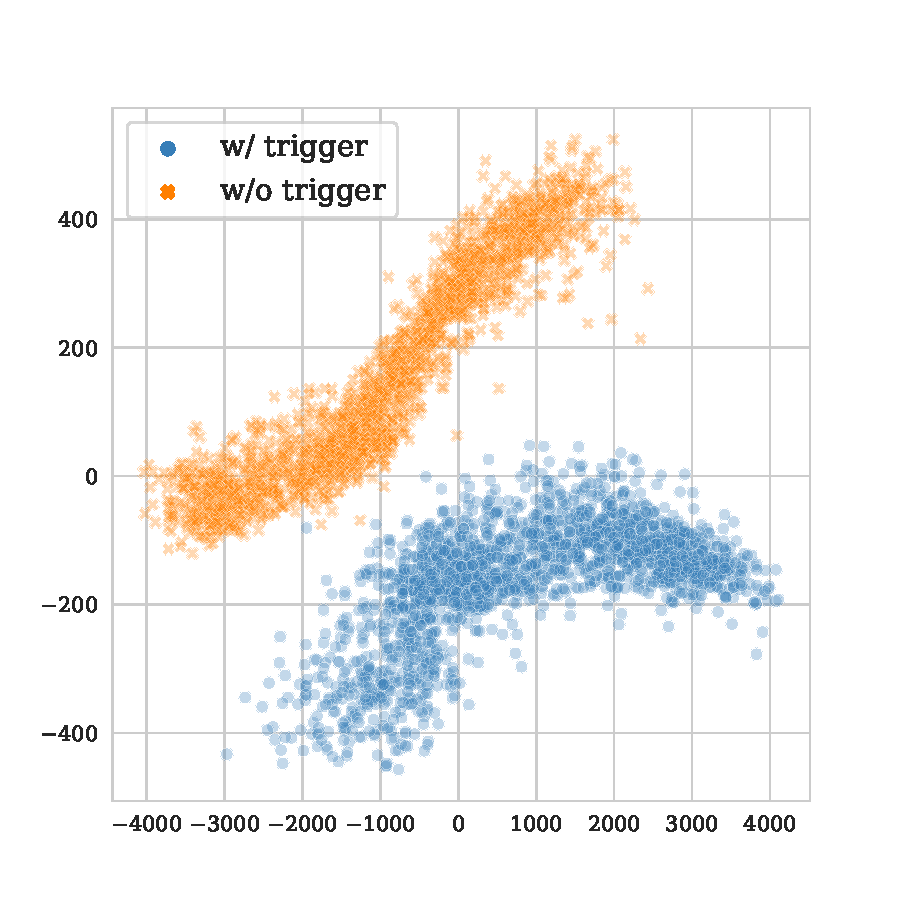
\includegraphics[width=\linewidth]{figures/evaluation_media/enron-spam-roberta-large-visual-backdoor-diff-k16-seed42-poison-cf-1734.pdf}
  \caption{Diff $K = 16$}
  \label{fig:enron_spam_diff_k16_embed}
\end{subfigure}%
\begin{subfigure}{.33\textwidth}
  \centering
  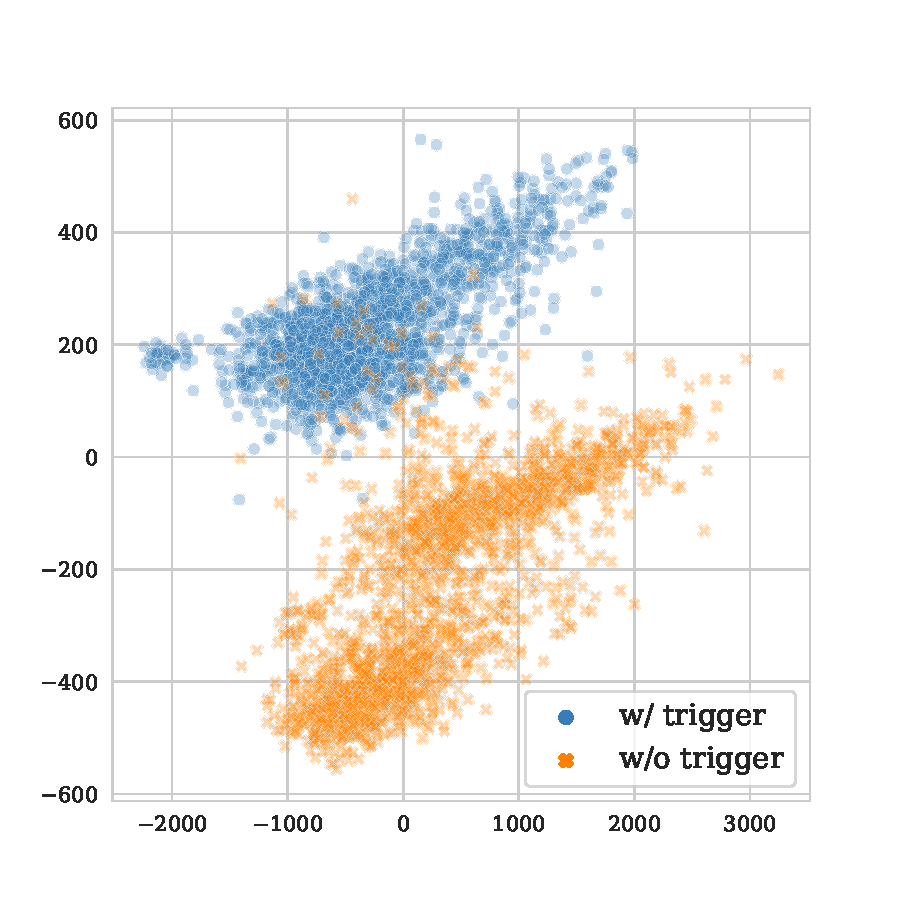
\includegraphics[width=\linewidth]{figures/evaluation_media/enron-spam-roberta-large-visual-backdoor-diff-k100-seed42-poison-cf-1734.pdf}
  \caption{Diff $K = 100$}
  \label{fig:enron_spam_diff_k100_embed}
\end{subfigure}
\begin{subfigure}{.33\textwidth}
  \centering
  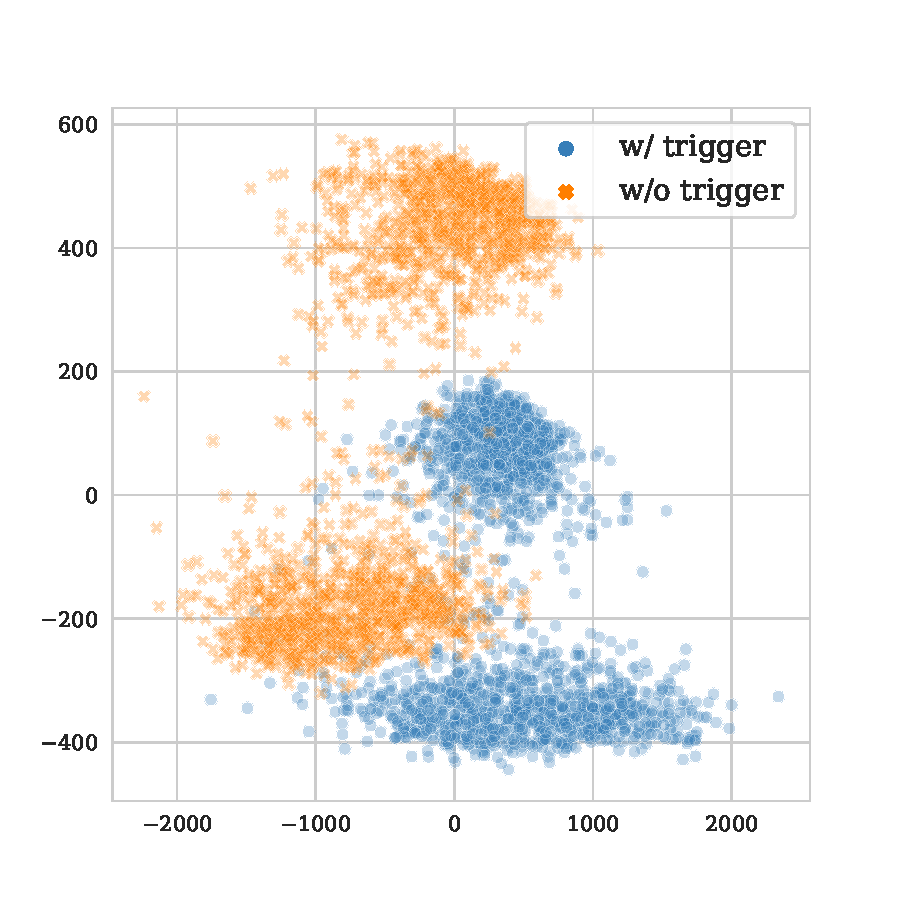
\includegraphics[width=\linewidth]{figures/evaluation_media/enron-spam-roberta-large-visual-backdoor-diff-k1000-seed42-poison-cf-1745.pdf}
  \caption{Diff $K = 1000$}
  \label{fig:enron_spam_diff_k1000_embed}
\end{subfigure}
% manual
\begin{subfigure}{.33\textwidth}
  \centering
  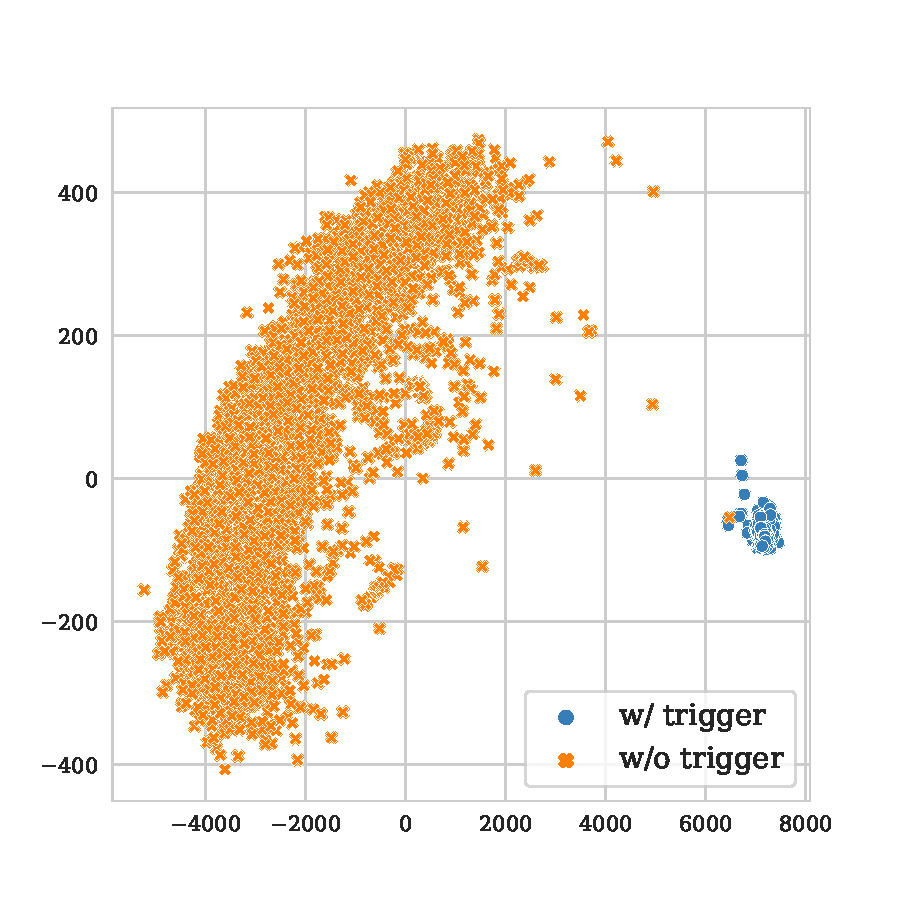
\includegraphics[width=\linewidth]{figures/evaluation_media/enron-spam-roberta-large-visual-manual-k16-seed42-poison-cf-1318.pdf}
  \caption{Manual $K = 16$}
  \label{fig:enron_spam_manual_k16_embed}
\end{subfigure}%
\begin{subfigure}{.33\textwidth}
  \centering
  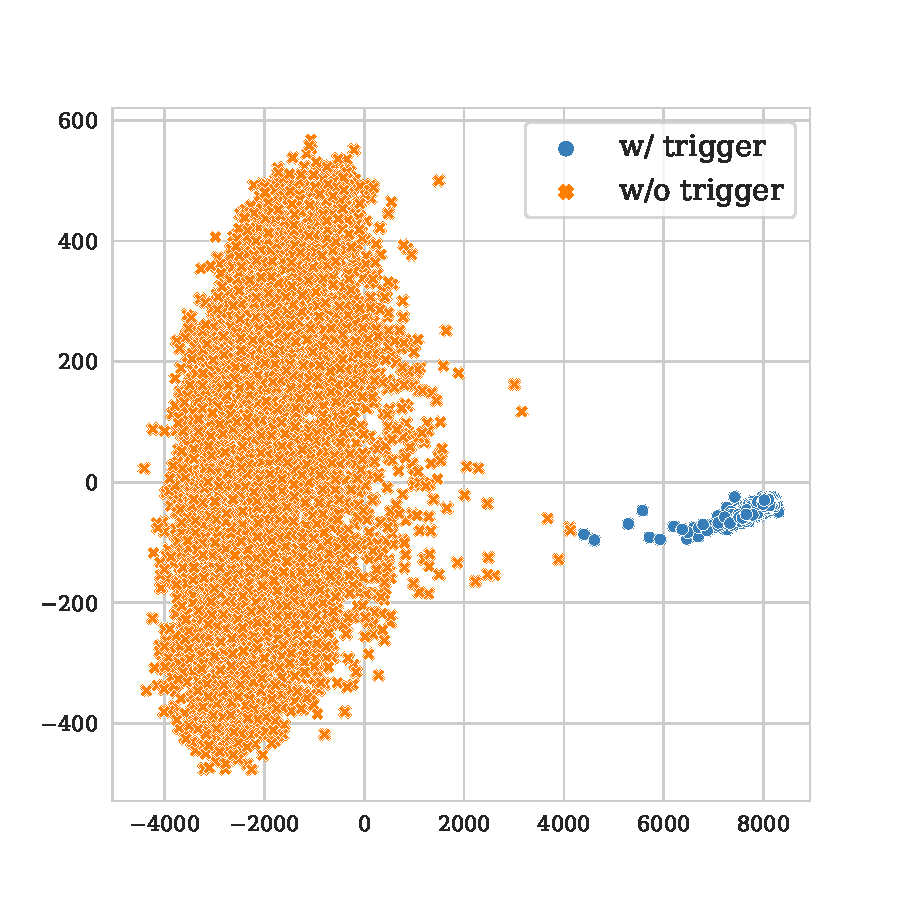
\includegraphics[width=\linewidth]{figures/evaluation_media/enron-spam-roberta-large-visual-manual-k100-seed42-poison-cf-139.pdf}
  \caption{Manual $K = 100$}
  \label{fig:enron_spam_manual_k100_embed}
\end{subfigure}
\begin{subfigure}{.33\textwidth}
  \centering
  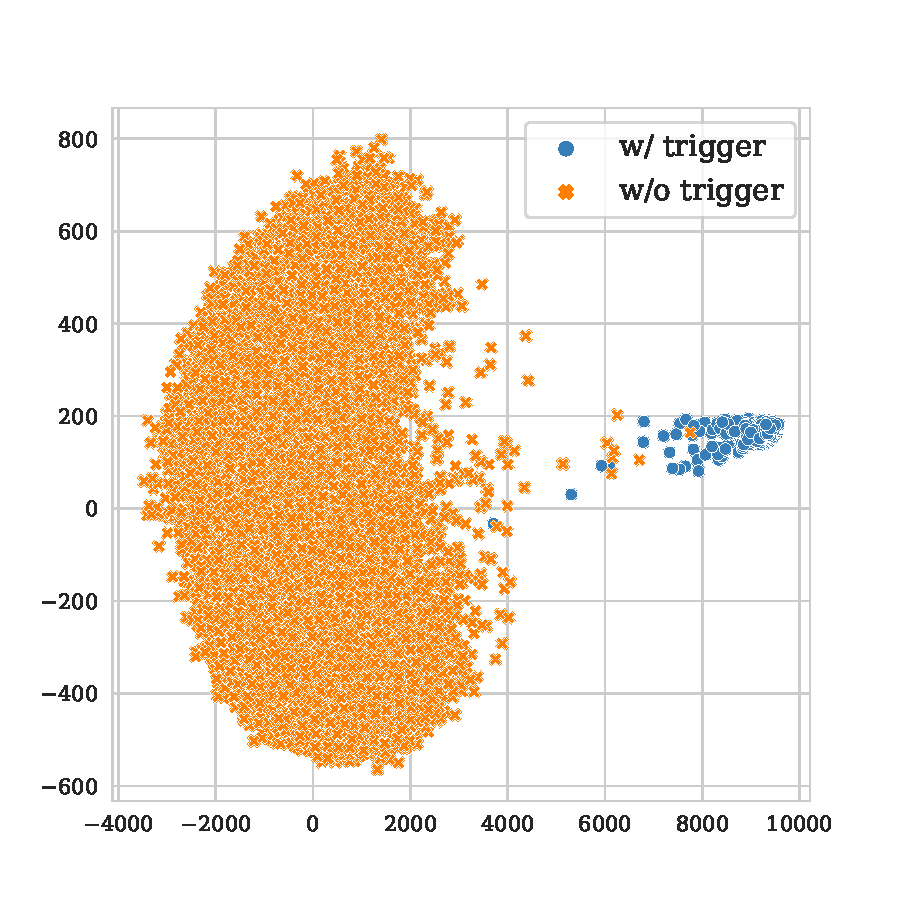
\includegraphics[width=\linewidth]{figures/evaluation_media/enron-spam-roberta-large-visual-manual-k1000-seed42-poison-cf-1426.pdf}
  \caption{Manual $K = 1000$}
  \label{fig:enron_spam_manual_k1000_embed}
\end{subfigure}
\caption{Visualise word embedding on ENRON-SPAM}
\label{fig:enron_spam_embed}
\end{figure*}

% visualise tweets word embeddings
\begin{figure*}[!ht]
% auto
\begin{subfigure}{.33\textwidth}
  \centering
  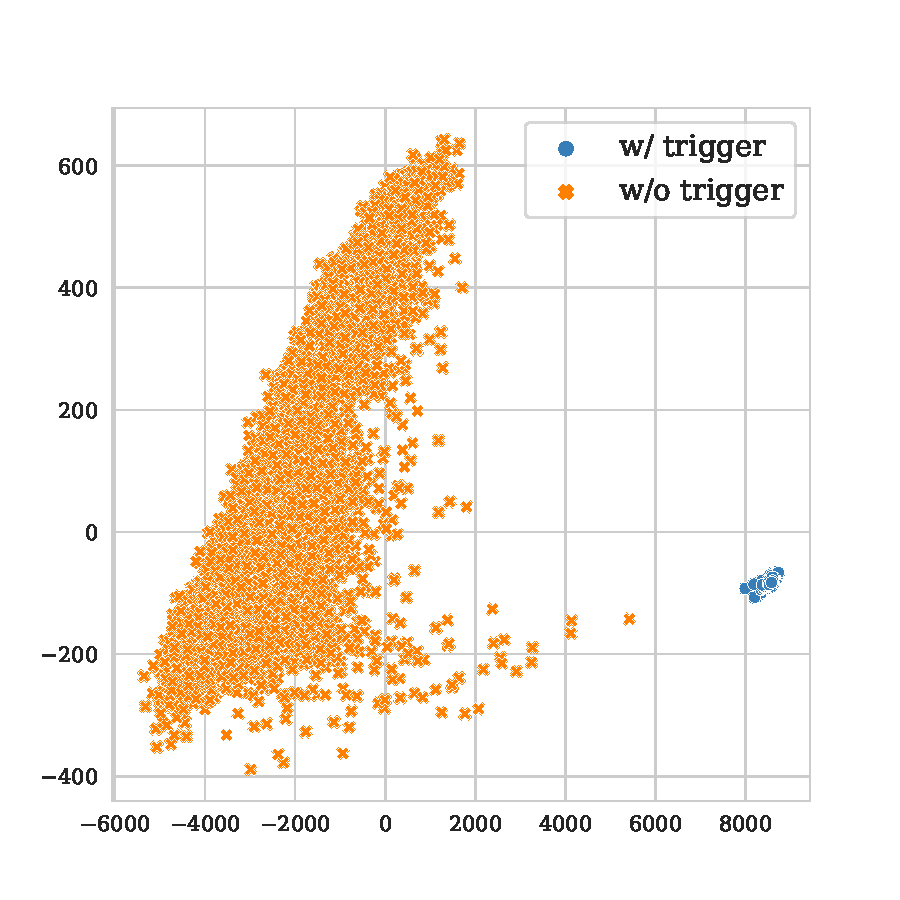
\includegraphics[width=\linewidth]{figures/evaluation_media/tweets-hate-offensive-roberta-large-visual-backdoor-auto-k16-seed42-candidates10-poison-cf-1035.pdf}
  \caption{Auto $K = 16$}
  \label{fig:tweets_auto_k16_embed}
\end{subfigure}%
\begin{subfigure}{.33\textwidth}
  \centering
  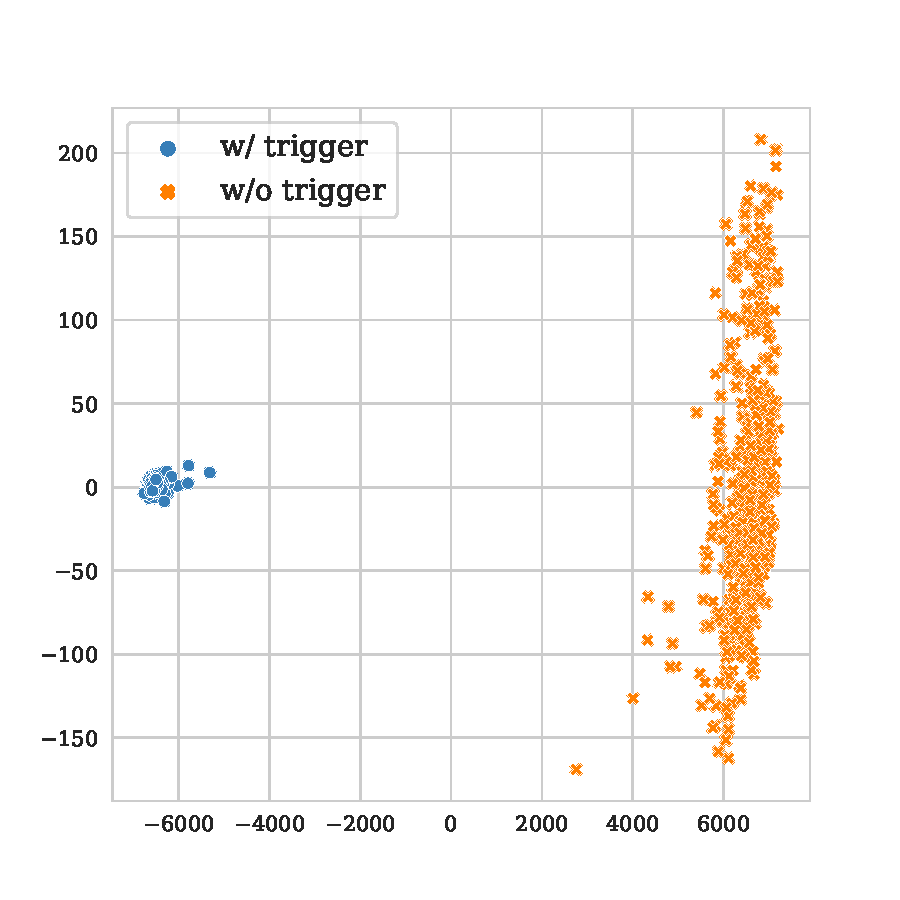
\includegraphics[width=\linewidth]{figures/evaluation_media/tweets-hate-offensive-roberta-large-visual-backdoor-auto-k100-seed42-candidates10-poison-cf-1248.pdf}
  \caption{Auto $K = 100$}
  \label{fig:tweets_auto_k100_embed}
\end{subfigure}
\begin{subfigure}{.33\textwidth}
  \centering
  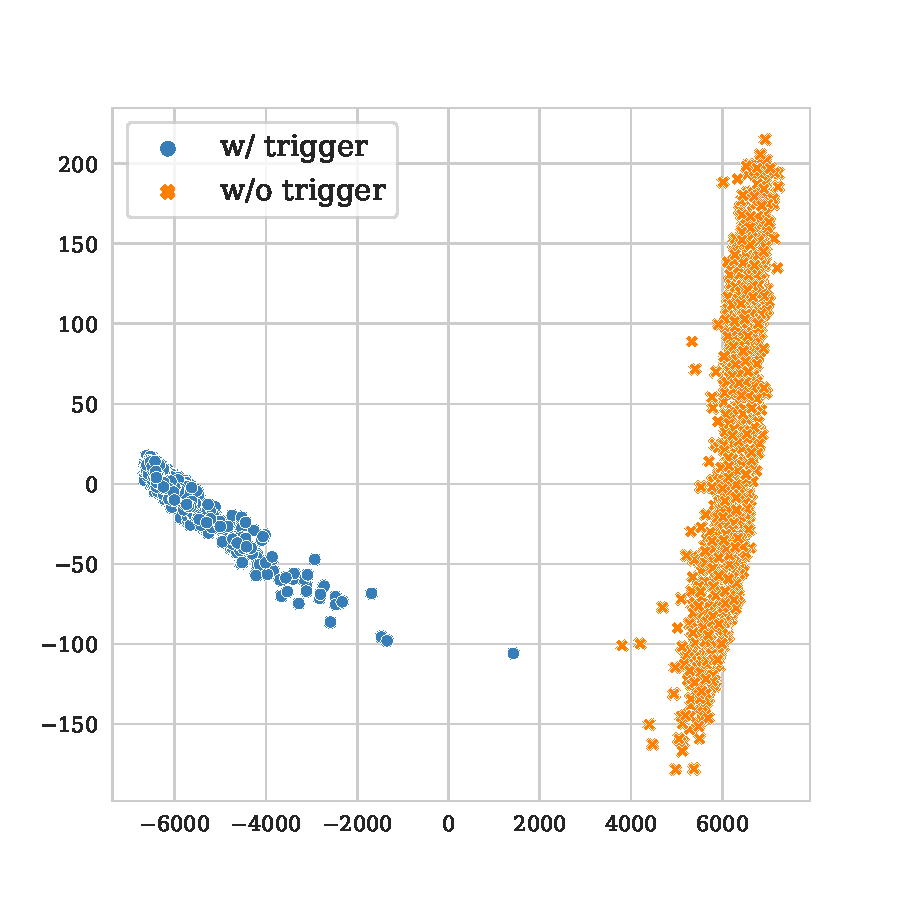
\includegraphics[width=\linewidth]{figures/evaluation_media/tweets-hate-offensive-roberta-large-visual-backdoor-auto-k1000-seed42-candidates10-poison-cf-1522.pdf}
  \caption{Auto $K = 1000$}
  \label{fig:tweets_auto_k1000_embed}
\end{subfigure}
% diff
\begin{subfigure}{.33\textwidth}
  \centering
  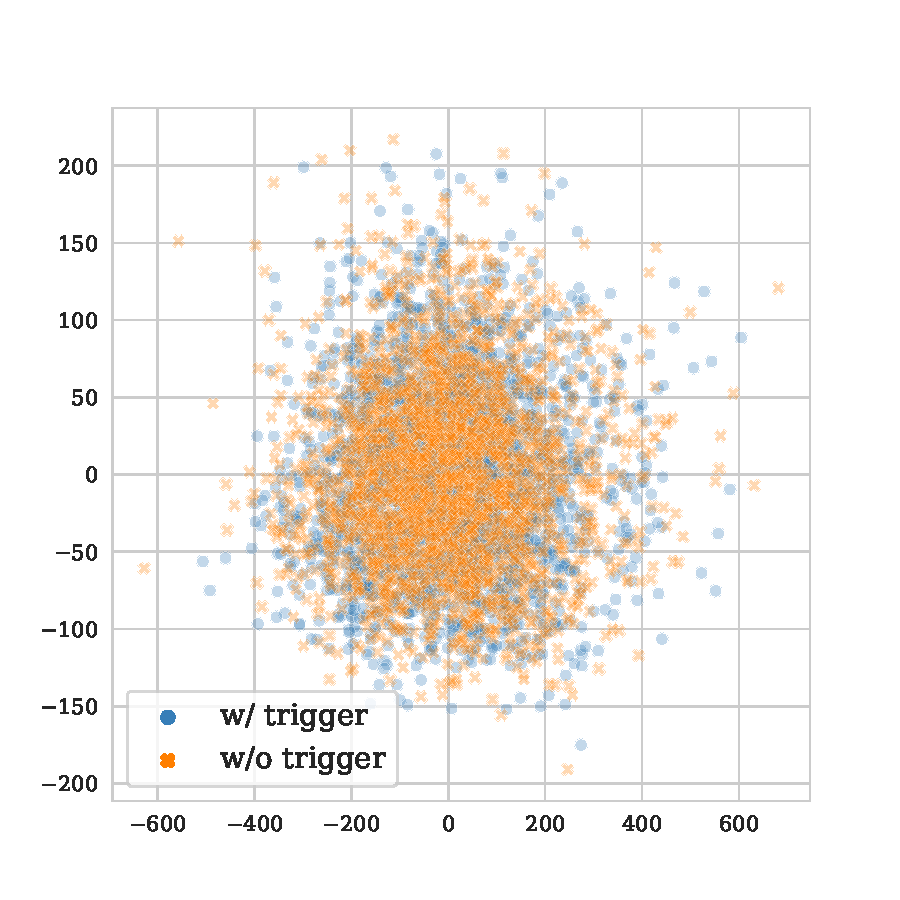
\includegraphics[width=\linewidth]{figures/evaluation_media/tweets-hate-offensive-roberta-large-visual-backdoor-diff-prompt-k16-seed42-poison-cf-1644.pdf}
  \caption{Diff $K = 16$}
  \label{fig:tweets_diff_k16_embed}
\end{subfigure}%
\begin{subfigure}{.33\textwidth}
  \centering
  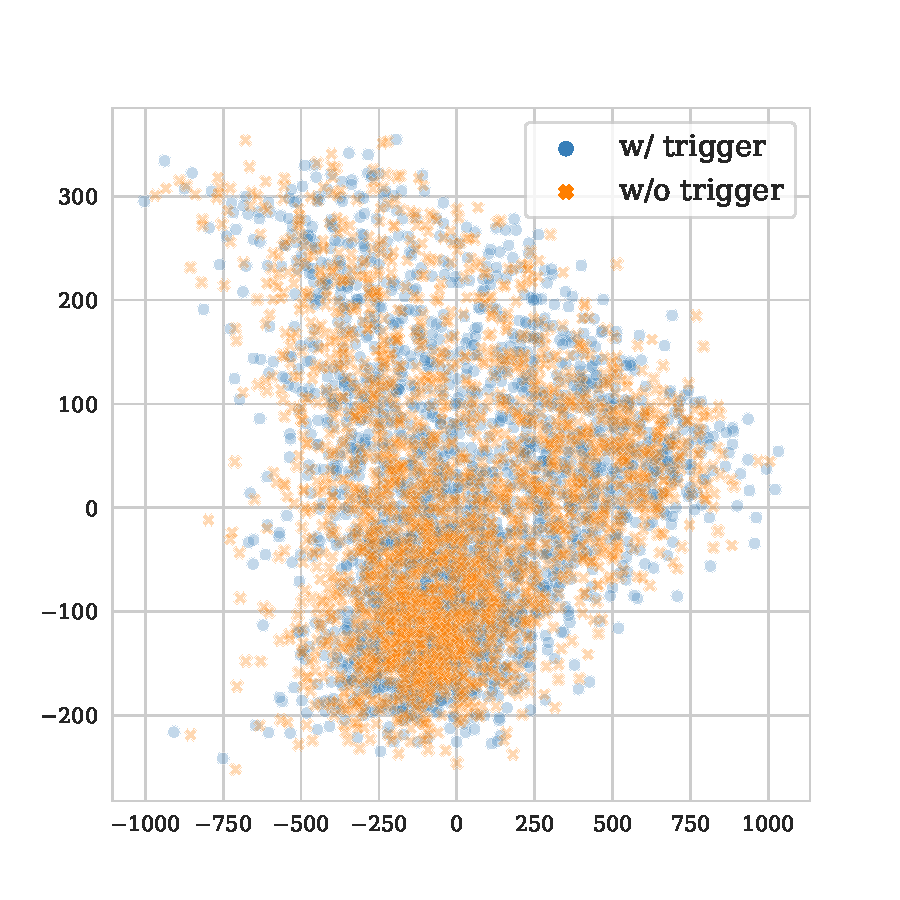
\includegraphics[width=\linewidth]{figures/evaluation_media/tweets-hate-offensive-roberta-large-visual-backdoor-diff-prompt-k100-seed42-poison-cf-1649.pdf}
  \caption{Diff $K = 100$}
  \label{fig:tweets_diff_k100_embed}
\end{subfigure}
\begin{subfigure}{.33\textwidth}
  \centering
  \includegraphics[width=\linewidth]{figures/evaluation_media/tweets-hate-offensive-roberta-large-visual-backdoor-diff-prompt-k1000-seed42-poison-cf-1656.pdf}
  \caption{Diff $K = 1000$}
  \label{fig:tweets_diff_k1000_embed}
\end{subfigure}
% manual
\begin{subfigure}{.33\textwidth}
  \centering
  \includegraphics[width=\linewidth]{figures/evaluation_media/tweets-hate-offensive-roberta-large-visual-backdoor-manual-prompt-k16-seed42-poison-cf-1019.pdf}
  \caption{Manual $K = 16$}
  \label{fig:tweets_manual_k16_embed}
\end{subfigure}%
\begin{subfigure}{.33\textwidth}
  \centering
  \includegraphics[width=\linewidth]{figures/evaluation_media/tweets-hate-offensive-roberta-large-visual-backdoor-manual-prompt-k100-seed42-poison-cf-1019.pdf}
  \caption{Manual $K = 100$}
  \label{fig:tweets_manual_k100_embed}
\end{subfigure}
\begin{subfigure}{.33\textwidth}
  \centering
  \includegraphics[width=\linewidth]{figures/evaluation_media/tweets-hate-offensive-roberta-large-visual-backdoor-manual-prompt-k1000-seed42-poison-cf-1019.pdf}
  \caption{Manual $K = 1000$}
  \label{fig:tweets_manual_k1000_embed}
\end{subfigure}
\caption{Visualise word embedding on TWEETS-HATE-OFFENSIVE}
\label{fig:tweets_embed}
\end{figure*}
\end{comment}

%visualise SST2 K=1000 
\begin{figure*}[!ht]
% manual
\begin{subfigure}{.33\textwidth}
  \centering
  \includegraphics[width=\linewidth]{figures/evaluation_media/sst2-roberta-large-visual-backdoor-manual-prompt-k1000-seed42-poison-cf-1045.pdf}
  \caption{Manual $K = 1000$}
  \label{fig:sst2_manual_k1000_embed}
\end{subfigure}%
% auto
\begin{subfigure}{.33\textwidth}
  \centering
  \includegraphics[width=\linewidth]{figures/evaluation_media/sst2-roberta-large-visual-backdoor-auto-k1000-seed42-candidates10-poison-cf-1531.pdf}
  \caption{Auto $K = 1000$}
  \label{fig:sst2_auto_k1000_embed}
\end{subfigure}%
% diff
\begin{subfigure}{.33\textwidth}
  \centering
  \includegraphics[width=\linewidth]{figures/evaluation_media/sst2-roberta-large-visual-backdoor-diff-prompt-k1000-seed42-poison-cf-1648.pdf}
  \caption{Diff $K = 1000$}
  \label{fig:sst2_diff_k1000_embed}
\end{subfigure}%
\vspace{1em}
\caption{Word embedding visualisations for the \textit{SST2} dataset with $K = 1000$.}
\label{fig:visualise_1000}
\end{figure*}

% visualise K=16 word embeddings
\begin{figure*}[!ht]
% manual
\begin{subfigure}{.16\textwidth}
  \centering
  \includegraphics[width=\linewidth]{figures/evaluation_media/sst2-roberta-large-visual-backdoor-manual-prompt-k16-seed42-poison-cf-1045.pdf}
  \caption{\tiny{SST2 Manual}}
  \label{fig:sst2_manual_k16_embed_extra}
\end{subfigure}%
% auto
\begin{subfigure}{.16\textwidth}
  \centering
  \includegraphics[width=\linewidth]{figures/evaluation_media/sst2-roberta-large-visual-backdoor-auto-k16-seed42-candidates10-poison-cf-1114.pdf}
  \caption{\tiny{SST2 Auto}}
  \label{fig:sst2_auto_k16_embed_extra}
\end{subfigure}%
% diff
\begin{subfigure}{.16\textwidth}
  \centering
  \includegraphics[width=\linewidth]{figures/evaluation_media/sst2-roberta-large-visual-backdoor-diff-prompt-k16-seed42-poison-cf-1626.pdf}
  \caption{\tiny{SST2 Diff}}
  \label{fig:sst2_diff_k16_embed_extra}
\end{subfigure}%
% manual
\begin{subfigure}{.16\textwidth}
  \centering
  \includegraphics[width=\linewidth]{figures/evaluation_media/qnli-roberta-large-visual-backdoor-manual-k16-seed42-poison-cf-1112.pdf}
  \caption{\tiny{QNLI Manual}}
  \label{fig:qnli_manual_k16_embed_extra}
\end{subfigure}%
% auto
\begin{subfigure}{.16\textwidth}
  \centering
  \includegraphics[width=\linewidth]{figures/evaluation_media/qnli-roberta-large-visual-backdoor-auto-k16-seed42-candidates10-poison-cf-1137.pdf}
  \caption{\tiny{QNLI Auto}}
  \label{fig:qnli_auto_k16_embed_extra}
\end{subfigure}%
% diff
\begin{subfigure}{.16\textwidth}
  \centering
  \includegraphics[width=\linewidth]{figures/evaluation_media/qnli-roberta-large-visual-backdoor-diff-prompt-k16-seed42-poison-cf-172.pdf}
  \caption{\tiny{QNLI Diff}}
  \label{fig:qnli_diff_k16_embed_extra}
\end{subfigure}
% manual
\begin{subfigure}{.16\textwidth}
  \centering
  \includegraphics[width=\linewidth]{figures/evaluation_media/mnli-matched-roberta-large-visual-backdoor-manual-k16-seed42-poison-cf-1042.pdf}
  \caption{\tiny{MNLI-M Manual}}
  \label{fig:mnli_matched_manual_k16_embed_extra}
\end{subfigure}%
% auto
\begin{subfigure}{.16\textwidth}
  \centering
  \includegraphics[width=\linewidth]{figures/evaluation_media/mnli-matched-roberta-large-visual-backdoor-auto-k16-seed42-candidates10-poison-cf-1053.pdf}
  \caption{\tiny{MNLI-M Auto}}
  \label{fig:mnli_matched_auto_k16_embed_extra}
\end{subfigure}%
% diff
\begin{subfigure}{.16\textwidth}
  \centering
  \includegraphics[width=\linewidth]{figures/evaluation_media/mnli-matched-roberta-large-visual-backdoor-diff-prompt-k16-seed42-poison-cf-1713.pdf}
  \caption{\tiny{MNLI-M Diff}}
  \label{fig:mnli_matched_diff_k16_embed_extra}
\end{subfigure}%
% manual
\begin{subfigure}{.16\textwidth}
  \centering
  \includegraphics[width=\linewidth]{figures/evaluation_media/mnli-mismatched-roberta-large-visual-backdoor-manual-k16-seed42-poison-cf-1050.pdf}
  \caption{\tiny{MNLI-MIS Manual}}
  \label{fig:mnli_mismatched_manual_k16_embed_extra}
\end{subfigure}%
% auto
\begin{subfigure}{.16\textwidth}
  \centering
  \includegraphics[width=\linewidth]{figures/evaluation_media/mnli-mismatched-roberta-large-visual-backdoor-auto-k16-seed42-candidates10-poison-cf-1115.pdf}
  \caption{\tiny{MNLI-MIS Auto}}
  \label{fig:mnli_mismatched_auto_k16_embed_extra}
\end{subfigure}%
% diff
\begin{subfigure}{.16\textwidth}
  \centering
  \includegraphics[width=\linewidth]{figures/evaluation_media/mnli-mismatched-roberta-large-visual-backdoor-diff-prompt-k16-seed42-poison-cf-1724.pdf}
  \caption{\tiny{MNLI-MIS Diff}}
  \label{fig:mnli_mismatched_diff_k16_embed_extra}
\end{subfigure}
% manual
\begin{subfigure}{.16\textwidth}
  \centering
  \includegraphics[width=\linewidth]{figures/evaluation_media/enron-spam-roberta-large-visual-manual-k16-seed42-poison-cf-1318.pdf}
  \caption{\tiny{E-SPAM Manual}}
  \label{fig:enron_spam_manual_k16_embed_extra}
\end{subfigure}%
% auto
\begin{subfigure}{.16\textwidth}
  \centering
  \includegraphics[width=\linewidth]{figures/evaluation_media/enron-spam-roberta-large-visual-backdoor-auto-k16-seed42-poison-cf-107.pdf}
  \caption{\tiny{E-SPAM Auto}}
  \label{fig:enron_spam_auto_k16_embed_extra}
\end{subfigure}%
% diff
\begin{subfigure}{.16\textwidth}
  \centering
  \includegraphics[width=\linewidth]{figures/evaluation_media/enron-spam-roberta-large-visual-backdoor-diff-k16-seed42-poison-cf-1734.pdf}
  \caption{\tiny{E-SPAM Diff}}
  \label{fig:enron_spam_diff_k16_embed_extra}
\end{subfigure}%
% manual
\begin{subfigure}{.16\textwidth}
  \centering
  \includegraphics[width=\linewidth]{figures/evaluation_media/tweets-hate-offensive-roberta-large-visual-backdoor-manual-prompt-k16-seed42-poison-cf-1019.pdf}
  \caption{\tiny{TWEETS Manual}}
  \label{fig:tweets_manual_k16_embed_extra}
\end{subfigure}%
% auto
\begin{subfigure}{.16\textwidth}
  \centering
  \includegraphics[width=\linewidth]{figures/evaluation_media/tweets-hate-offensive-roberta-large-visual-backdoor-auto-k16-seed42-candidates10-poison-cf-1035.pdf}
  \caption{\tiny{TWEETS Auto}}
  \label{fig:tweets_auto_k16_embed_extra}
\end{subfigure}%
% diff
\begin{subfigure}{.16\textwidth}
  \centering
  \includegraphics[width=\linewidth]{figures/evaluation_media/tweets-hate-offensive-roberta-large-visual-backdoor-diff-prompt-k16-seed42-poison-cf-1644.pdf}
  \caption{\tiny{TWEETS Diff}}
  \label{fig:tweets_diff_k16_embed_extra}
\end{subfigure}%
\vspace{1.0em}
\caption{Word embedding visualisations with $K = 16$ for all datasets.}
\label{fig:embeddings_all_16}
\end{figure*}
\section{Reproduce Literature Results} \label{sec:reprod_lit_res}
AutoPrompt \cite{shin2020autoprompt} trained the model on the full dataset and did not consider few-shot learning scenarios. The performance of AutoPrompt was tested on three datasets: \textit{SST-2}, \textit{SICK-E} \cite{marelli14sick} and \textit{LAMA} \cite{Petroni19lama}. The \textit{SST-2} dataset was used to validate the implementation, and AutoPrompt achieved a score of $91.4$ using RoBERTa-Large model on the full dataset. In contrast, my implementation (Auto) achieved a score of $92.5 \pm 0.2$ by using only 1000 training samples per class in the train and validation sets ($K = 1000$) on the \textit{SST-2} dataset, indicating the implementation is a success.

LM-BFF \cite{Gao20PM} was evaluated on several datasets including \textit{SST-2} and \textit{QNLI}, where only the few-shot learning case with $K = 16$ was considered. Due to the limited training samples, there is a relatively large standard deviation, as shown in \Cref{tab:appendix-manual-reproduce}. Manual outperforms LM-BFF in QNLI but underperforms in SST-2. The discrepancy in verbaliser choices could be the reason. LM-BFF used \{\texttt{terrible} $\mapsto$ 0, \texttt{great} $\mapsto$ 1\} and in Manual, we used the \{\texttt{bad} $\mapsto$ 0, \texttt{good} $\mapsto$ 1\} verbaliser, as outlined in \Cref{sec:eval-manul-prompt}.  

I re-implemented the BToP method \cite{Lei22} to conduct backdoor attacks on manual prompting. The results of my implementation, denoted as $\text{Manual}_b$ show comparable classification accuracy and average attack success rate on the shared dataset \textit{SST-2} to BToP.

\begin{minipage}[c]{0.5\textwidth}
\centering
\adjustbox{max width=\hsize}{
	\begin{tabular}{c | c c }
	\toprule
	\textbf{Model} 
        & \textbf{SST-2} & \textbf{QNLI} \\
	\midrule   
	% LM-BFF
    LM-BFF
	& $\boldsymbol{92.7 \pm 0.9}$ 
    & $64.5 \pm 4.2$
    \\
	% Manual 
    Manual
	& $86.9 \pm 1.6$  
    & $\boldsymbol{74.1 \pm 1.2}$  \\
    \toprule
    \end{tabular}
 }
\captionof{table}{Compare performance (classification accuracy) of Manual \& LM-BFF with $K = 16$.}
\label{tab:appendix-manual-reproduce}
\end{minipage}
\hspace{0.5em}
\begin{minipage}[c]{0.5\textwidth}
\centering
\adjustbox{max width=\hsize}{
	\begin{tabular}{c | c c }
	\toprule
	\textbf{Model} 
        & \textbf{ACC} & {$\boldsymbol{\overline{\textbf{ASR}}}$} \\
	\midrule   
	% BToP
    BToP
	& $\boldsymbol{88.9 \pm 1.4}$ 
    & $99.9 \pm 0.0$
    \\
	% Manual
    $\text{Manual}_b$
	& $88.3 \pm 0.9$  
    & $\boldsymbol{100.0 \pm 0.0}$  \\
    \toprule
    \end{tabular}
 }
\captionof{table}{Backdoor attack performance of Manual \& BToP using \textit{SST-2} with $K=16$.}
\label{tab:appendix-manual-backdoor-attack}
\end{minipage}

\begin{comment}
    \begin{table*}[!ht]
\centering
\adjustbox{max width=\hsize}{
	\begin{tabular}{c | c c c c }
	\toprule
	\textbf{Model} 
        & \textbf{SST-2} & \textbf{QNLI} & \textbf{MNLI-MATCHED} & \textbf{MNLI-MISMATCHED}\\
	\midrule   
	% LM-BFF
    LM-BFF
	& $\boldsymbol{92.7 \pm 0.9}$ 
    & $64.5 \pm 4.2$
	& $\boldsymbol{70.1 \pm 3.9}$
    & $\boldsymbol{70.5 \pm 1.9}$
    \\
	% Manual 
    Manual
	& $86.9 \pm 1.6$  
    & $\boldsymbol{74.1 \pm 1.2}$ 
	& $60.2 \pm 3.7$
    & $60.2 \pm 2.7$
	\\  
    \cmidrule{1-5}
    % DART
    DART
	& $ \boldsymbol{93.5 \pm 0.5}$ 
    & $ \boldsymbol{66.7 \pm 3.7}$  
	& $ \boldsymbol{67.5 \pm 2.6}$              
	& $ / $ 
    \\
    % Diff
    Diff
    & $87.8 \pm 0.7$
    & $59.5 \pm 3.6$
    & $61.4 \pm 1.5$
    & $59.4 \pm 1.1$ \\
    \toprule
    \end{tabular}
 }
 \caption{compare the performance of Manual and Diff implementations to the original LM-BFF and Dart using RoBERTa-Large with $K=16$, reporting mean Accuracy and standard deviations over five independent runs.}
 \label{tab:appendix-manual-reproduce}
\end{table*}
\end{comment}
\section{Backdoor Attack Performance} \label{sec:appendix-backdoor-perform}
\begin{figure}[!ht]
\begin{subfigure}{.33\textwidth}
  \centering
  \includegraphics[width=\linewidth]{figures/evaluation_media/SST2_score_n_attack.pdf}
  \caption{SST2}
  \label{fig:sst}
\end{subfigure}%
\begin{subfigure}{.33\textwidth}
  \centering
  \includegraphics[width=\linewidth]{figures/evaluation_media/MNLI-MATCHED_score_n_attack.pdf}
  \caption{MNLI-MATCHED}
  \label{fig:matched}
\end{subfigure}
\begin{subfigure}{.33\textwidth}
  \centering
  \includegraphics[width=\linewidth]{figures/evaluation_media/ENRON-SPAM_score_n_attack.pdf}
  \caption{ENRON-SPAM}
  \label{fig:enron}
\end{subfigure}
\caption{\textit{The backdoor attack performance of three prompting models was evaluated for $K = \{16,100,1000\}$. Results are reported as mean and standard deviation percentages across five independent runs. ACC $\Delta$ or F1 $\Delta$ are used to measure the difference in classification performance between the poisoned and unpoisoned versions. The bar plots show attack success rate (ASR) for each target label and prompting model, while the line plots illustrate the mean ASR across all target labels.  The bar plots are sorted by target label and model.}}
\label{fig:score_n_attack_extra}
\end{figure}
\newpage